% Modified for use with Wiley Interdisciplinary Reviews Copyright (C) (2016). All rights reserved.
\documentclass[12pt]{article}

\setlength{\oddsidemargin}{0in}  %left margin position, reference is one inch
\setlength{\textwidth}{6.5in}    %width of text=8.5-1in-1in for margin
\setlength{\topmargin}{-0.5in}    %reference is at 1.5in, -.5in gives a start of about 1in from top
\setlength{\textheight}{9in}     %length of text=11in-1in-1in (top and bot. marg.) 
\usepackage{longtable}
\usepackage{amsmath,amssymb}
\usepackage{graphicx}% Include figure files
\usepackage[skip=8pt]{caption}
\usepackage{enumitem}
\usepackage{scalerel}
\usepackage{multirow}
\usepackage{color}% Include colors for document elements
\usepackage{dcolumn}% Align table columns on decimal point
\usepackage{bm}% bold math
\usepackage{float}
\usepackage{hyperref} % hyperref must be loaded before apacite
\usepackage{apacite}
\usepackage{arydshln, newfloat}
\usepackage{multicol}
\bibliographystyle{apacite} 
\usepackage{caption}
\usepackage{subfig}
\usepackage{booktabs}
\newcommand{\hilbert}{\mathcal{H}}
\newcommand{\argmin}[1]{\underset{#1}{\operatorname{arg}\,\operatorname{min}}\;}
\newcommand{\hilbertl}{\mathcal{H}_{\langle l \rangle}}
\newcommand{\hilbertm}{\mathcal{H}_{\langle m \rangle}}
\newcommand{\hilbertlnull}{\mathcal{H}_{0\langle l \rangle}}
\newcommand{\hilbertmnull}{\mathcal{H}_{0\langle m \rangle}}
\newcommand{\hilbertlpen}{\mathcal{H}_{1\langle l \rangle}}
\newcommand{\hilbertmpen}{\mathcal{H}_{1\langle m \rangle}}
\newcommand{\PP}{\mathcal{P}}
\newcommand{\vphistar}{\mbox{\boldmath $\phi$}}
\newcommand{\vsigmasq}{\mbox{\boldmath $\sigma^2$}}
\newcommand{\bfeps}{\mbox{\boldmath $\epsilon$}}
\newcommand{\bfgamma}{\mbox{\boldmath $\gamma$}}
\newcommand{\bflam}{\mbox{\boldmath $\lambda$}}
\newcommand{\bfphi}{\mbox{\boldmath $\phi$}}
\newcommand{\bfsigma}{\mbox{\boldmath $\sigma$}}
\newcommand{\bfkappa}{\mbox{\boldmath $\kappa$}}
\newcommand{\bfbeta}{\mbox{\boldmath $\beta$}}
\newcommand{\bfalpha}{\mbox{\boldmath $\alpha$}}
\newcommand{\bftheta}{\mbox{\boldmath $\theta$}}
\newcommand{\bfe}{\mbox{\boldmath $e$}}
\newcommand{\bft}{\mbox{\boldmath $t$}}
\newcommand{\bfg}{\mbox{\boldmath $g$}}
\newcommand{\bfv}{\mbox{\boldmath $v$}}
\newcommand{\bfu}{\mbox{\boldmath $u$}}
\newcommand{\bfx}{\mbox{\boldmath $x$}}
\newcommand{\bfy}{\mbox{\boldmath $y$}}
\newcommand{\bff}{\mbox{\boldmath $f$}}
\newcommand{\bfone}{\mbox{\boldmath $1$}}
\newcommand{\bfo}{\mbox{\boldmath $0$}}
\newcommand{\bfO}{\mbox{\boldmath $O$}}
\newcommand{\bfX}{\mbox{\boldmath $X$}}
\newcommand{\bfz}{\mbox{\boldmath $z$}}
\newcommand{\tildeY}{\tilde{Y}}
\newcommand{\tildey}{\tilde{y}}
\newcommand{\tildeQ}{\tilde{Q}}
\newcommand{\tildeK}{\tilde{K}}
\newcommand{\tildeR}{\tilde{R}}
\newcommand{\tildeA}{\tilde{A}}
\newcommand{\tildeepsilon}{\tilde{\epsilon}}
\newcommand{\bfepsilon}{\mbox{\boldmath $\epsilon$}}
\newcommand{\tildeS}{\tilde{S}}

\newcommand{\bfm}{\mbox{\boldmath $m$}}
\newcommand{\bfa}{\mbox{\boldmath $a$}}
\newcommand{\bfb}{\mbox{\boldmath $b$}}
\newcommand{\bfY}{\mbox{\boldmath $Y$}}
\newcommand{\bfB}{\mbox{\boldmath $B$}}
\newcommand{\bfZ}{\mbox{\boldmath $Z$}}
\newcommand{\tildeB}{\tilde{B}}

\newtheorem{theorem}{Theorem}[section]
\newtheorem{lemma}[theorem]{Lemma}
\newtheorem{proposition}[theorem]{Proposition}
\newtheorem{corollary}[theorem]{Corollary}
\usepackage{bm}
\definecolor{wes1}{RGB}{216,183,10}
\definecolor{wes2}{RGB}{214,114,54}
\definecolor{wes3}{RGB}{2,64,27}
\definecolor{wes4}{RGB}{162,164 ,117}
\definecolor{wes5}{RGB}{129,168,141}
\captionsetup[figure]{font=small,labelfont=small}

\hypersetup{colorlinks = true, citecolor = black, urlcolor = blue}
%\usepackage[nolists, nomarkers, figuresfirst]{endfloat}


%%% added for editing -- lee
\usepackage{ulem}
\newcommand{\red}[1]{{\color{red}\sout{#1}}}
\newcommand{\blue}[1]{{\color{blue}#1}}
%%%%%%%%


\definecolor{background-color}{gray}{0.98}
\title{ Nonparametric covariance estimation with shrinkage toward stationary models }
% The title should not exceed 20 words. Please be original and try to include keywords, especially before a colon if applicable, as they will increase the discoverability of your article. Visit http://media.wiley.com/assets/7158/18/SEO_For_Authors.pdf for tips on search engine optimization.

\author{Tayler A. Blake\thanks{Department of Statistics, The Ohio State University, Columbus, OH, USA}  
\and Yoonkyung Lee\footnotemark[1]
%\thanks{Department of Statistics, The Ohio State University, Columbus, OH}
}
% The preferred (but optional) format for author names is First Name, Middle Initial, Last Name.
% Wiley requires that all authors disclose any potential conflicts of interest.  Any interest or relationship, financial or otherwise, that might be perceived as influencing an author’s objectivity is considered a potential conflict of interest. The existence of a conflict of interest does not preclude publication.
\DeclareCaptionType{InfoBox}
\date{}
\begin{document}
\maketitle
 
\begin{center}
\subsubsection*{\small Article Type:} Focus Article
%The Article Type denotes the intended level of readership for your article. An Editor may have mentioned a specific Article Type in your invitation letter; if so, please let them know if you think a different Article Type better suits your topic.

\hfill \break
\thanks

\subsubsection*{Abstract}
\begin{flushleft}
Estimation of an unstructured covariance matrix is difficult because of the challenges posed by parameter space dimensionality and the positive definiteness constraint that estimates should satisfy. We consider a general nonparametric covariance estimation framework for longitudinal data using the Cholesky decomposition of a positive-definite matrix. The covariance matrix of time-ordered measurements  is diagonalized by a lower triangular matrix with unconstrained entries that are statistically interpretable as parameters for a varying coefficient autoregressive model.  Using this dual interpretation of the Cholesky decomposition and allowing for irregular sampling time points, we treat covariance estimation as bivariate smoothing and cast it in a regularization framework for desired forms of simplicity in covariance models. 
Viewing stationarity as a form of simplicity or parsimony in covariance, we model  the varying coefficient function with components depending on time lag and  its orthogonal direction separately and penalize the components that capture the nonstationarity in the fitted function. We demonstrate construction of a covariance estimator using the smoothing spline framework. Simulation studies establish the advantage of our approach over alternative estimators proposed in the longitudinal data setting. We analyze a longitudinal dataset to illustrate application of the methodology and compare our estimates to those resulting from alternative models. 

%Estimation of an unstructured covariance matrix is difficult because of the challenges posed by parameter space dimensionality and the positive definiteness constraint that estimates should satisfy. We propose a general nonparametric covariance estimation framework for longitudinal data using the Cholesky decomposition of the covariance matrix. The covariance matrix is diagonalized by a lower triangular matrix with unconstrained entries, which is treated as a smooth bivariate surface and approximated by tensor product splines. Through the use of the Cholesky decomposition, we illustrate the equivalence of covariance estimation and the estimation of a varying coefficient autoregressive model.

%\bigskip
%Viewing stationarity as a form of simplicity or parsimony in covariance models, we specify the varying coefficient as a function so that we can conveniently penalize the components which capture the nonstationarity in the fitted function. We demonstrate construction of a covariance estimator using the smoothing spline framework. Simulation studies establish the advantage of our approach over alternative estimators proposed in the longitudinal data setting. We analyze a longitudinal dataset to illustrate application of the methodology and compare our estimates to those resulting from alternative models proposed for the covariance for longitudinal data. 
\end{flushleft}
\end{center}


\clearpage

\renewcommand{\baselinestretch}{1.5}
\normalsize

\clearpage

\section*{\sffamily \Large GRAPHICAL TABLE OF CONTENTS} 
%Include an attractive full color image for the online Table of Contents. It may be a figure or panel from the article, or may be specifically designed as a visual summary. You will need to upload this as a separate file during submission.
%
%Size: The maximum width and height are 390 pixels, and the minimum resolution is 300 dpi. Multi-panel graphs or images are strongly discouraged.
%
%Caption: This is a narrative sentence to convey the article's essence and wider implications to a non-specialist audience. The maximum length is 50 words, but consider using 140 characters or less to facilitate social media sharing, which can increase the discoverability of your article.

\section*{\sffamily \Large INTRODUCTION} 

%Introduce your topic in around 2 paragraphs, around 750 words.  Please define all acronyms at their first usage except IR, UV, NMR, DNA or similar commonly understood terms.  References should use the \href{http://www.apastyle.org/learn/quick-guide-on-references.aspx}{APA style}, like this \cite{coulson1960present}.


Estimation of a  covariance matrix is fundamental to the analysis of multivariate data for mean inference, discrimination, and dimension reduction. The two primary challenges in fulfilling this prerequisite are due to the total number of parameters to be estimated in relation to the data dimension, and a structural constraint for covariance. As compared to mean estimation, the number of parameters grows quadratically in the dimension, and these parameters must satisfy the positive-definiteness constraint. It is well known that the widely used the sample covariance matrix, though positive-definite and unbiased for the population covariance matrix, is unstable in high dimensions \cite{lin1985monte,johnstone2001distribution}. In the applied literature, it is common practice to specify a parametric model for the covariance structure by incorporating primary factors for variation in the data or those elements suggested by a study design. These models are typically parsimonious and require modest computational effort for estimation. However, specifying the appropriate covariance model is challenging even for the experts, and model misspecification can lead to considerably biased estimates. 

On the other hand, several regularized estimators of the sample covariance have been proposed to balance the two extremes. There are several elementwise regularization methods for estimating a covariance matrix; see, for example, \citeA{bickel2008regularized,cai2010optimal,yao2005functional,rothman2009generalized}. Methods for covariance estimation leveraging elementwise shrinkage are attractive, in part, because they typically present very low computational burden, but such estimators are not guaranteed to be positive-definite with finite sample sizes.

There has been a recent shift in covariance estimation toward regression-based approaches to eliminate the positive-definite constraint from estimation procedures altogether.  Similar to this idea is the approach of modeling various matrix decompositions directly rather than the covariance matrix itself, including the spectral decomposition, the variance-correlation decomposition, and the Cholesky decomposition. The Cholesky decomposition in particular has recently received much attention because of its qualities that make it particularly attractive for its use in covariance estimation for data with naturally ordered measurements such as time series or longitudinal data. The entries of the lower triangular matrix and the diagonal matrix of the modified Cholesky decomposition have statistical interpretations as autoregressive coefficients, or the \textit{generalized autoregressive parameters} and prediction variances, or \textit{innovation variances}  when regressing a measurement on its predecessors. The unconstrained reparameterization and its statistical interpretability makes it easy to cast covariance modeling into the generalized linear model framework while guaranteeing that the resulting estimates are positive-definite. See \citeA{pourahmadi2011covariance} for a general overview of modeling the Cholesky decomposition.

In this paper, we extend the regression model associated with the Cholesky decomposition of a covariance matrix to a functional varying coefficient model. Treating covariance estimation as bivariate smoothing, our framework naturally accommodates unbalanced longitudinal data and employs regularization as in the usual function estimation setting. The outline of the article is as follows. In Section 2, we review the role of the modified Cholesky decomposition in the
unconstrained reparametrization of a covariance matrix. In Section 3, we present a functional varying coefficient model for the elements of the reparameterized covariance matrix and propose reproducing kernel Hilbert space framework for estimation of the varying coefficient function. We demonstrate estimation of the innovation variances via smoothing splines in Section 4. Section 5 reviews a simulation study comparing the performance of our estimator to other covariance estimators proposed in the literature, and we apply our method to a dataset collected from a longitudinal study of cattle weights in Section 6.  

\section*{\sffamily \Large THE CHOLESKY DECOMPOSITION}
% The Cholesky decomposition of a positive-definite matrix is given by
%\begin{equation}\label{eq:standard-cholesky-decomposition}
%\Sigma = CC',
%\end{equation}
%\noindent
%where $C = \left[c_{ij} \right]$ is a unique lower-triangular matrix with positive diagonal entries. Interpretation of the entries of $C$ is difficult in this form \cite{pinheiro1996unconstrained}. However, transforming $C$ to a unit lower-triangular matrix dividing the $i^{th}$ column of $C$ by its $i^{th}$ diagonal element $c_{ii}$ makes the statistical interpretation of the diagonal entries of $C$ and the resulting unit lower-triangular matrix much more straightforward. Letting $D^{1/2} = diag\left( c_{11},\dots, c_{pp} \right)$, the standard Cholesky decomposition \eqref{eq:standard-cholesky-decomposition} can be written
%\begin{equation}\label{eq:standard-cholesky-decomposition-transform}
%\Sigma = CD^{-1/2}DD^{-1/2}C' = L D L',
%\end{equation}
%\noindent
%where $L = D^{-1/2}C$. 

For a positive-definite covariance matrix $\Sigma \in \Bbb{R}^{p\times p}$ for $p$ variables, there exist a  lower triangular matrix $T \in \Bbb{R}^{p\times p}$ with unit diagonal entries and a diagonal matrix $D \in \Bbb{R}^{p\times p}$ with positive entries such that
\begin{equation}\label{eq:modified-cholesky-decomposition}
D = T\Sigma T'.
\end{equation}
 \noindent
%\red{where $D$ is a diagonal matrix with positive entries, and $T$ is a lower triangular matrix with diagonal entries equal to 1.} 
This representation \eqref{eq:modified-cholesky-decomposition} is commonly referred to as the modified Cholesky decomposition of $\Sigma$. 

The lower triangular entries of $T$ are unconstrained and can be interpreted as the coefficients of a particular regression model for ordered variables, and the diagonal of $D$ can be interpreted as the prediction error variances associated with the same model.  Let $Y = \left( y_1,\dots, y_p \right)'$ denote a mean zero random vector with positive-definite covariance matrix $\Sigma$, and consider regressing $y_t$ on its predecessors $y_1, \dots, y_{t-1}$. Let $\hat{y}_t$ be the linear least-squares predictor of $y_t$ based on previous measurements $y_{t-1}, \dots , y_1$, and let $Var\left(\epsilon_t\right) = \sigma_t^2$ denote the variance of the corresponding prediction error, where $\epsilon_t = y_t - \hat{y}_t$. Regression theory gives us that there exist unique scalars $\phi_{tj}$ so that
\begin{equation} \label{eq:mcd-ar-model}
y_t = \left\{ \begin{array}{ll} \epsilon_t, & t = 1\\
\sum_{j = 1}^{t-1} \phi_{tj} y_j + \epsilon_t, & t = 2, \dots, p,
\end{array}\right.
\end{equation}
\noindent
and the prediction errors $\epsilon_t$ are mean zero and independently distributed. If we negate the regression coefficients $\phi_{tj}$ and place them in the lower triangle of $T$ so that the $\left(t, j\right)$ entry of $T$ is $-\phi_{tj}$, and let $D = \mbox{diag}\left(\sigma^2_1, \dots, \sigma_p^2\right)$ and
$\epsilon = \left(\epsilon_1,\dots, \epsilon_p\right)'$, then the sequence of regression models in \eqref{eq:mcd-ar-model} can be written in matrix form as
\begin{equation} \label{eq:e-equals-T-Y}
\epsilon = TY.
\end{equation}
\noindent
The $\left(t, j\right)$ entry of $T$ is $-\phi_{tj}$, and $\sigma_t^2 = Var\left(\epsilon_t\right)$. 
Taking covariances on both sides of \eqref{eq:e-equals-T-Y} gives the modified Cholesky decomposition \eqref{eq:modified-cholesky-decomposition}; thus, modeling a covariance matrix is equivalent to fitting a sequence of $p - 1$ varying-coefficient and varying-order regression models.  Since the $\phi_{tj}$ are regression coefficients, these and the log variances $\log \sigma_t^2$ are unconstrained. The regression coefficients of the model in \eqref{eq:mcd-ar-model} are referred to as the \textit{generalized autoregressive parameters} and \textit{innovation variances} \cite{pourahmadi1999joint,pourahmadi2000maximum}. The powerful implication of the regression framework of decomposition \eqref{eq:modified-cholesky-decomposition} is the accessibility of the entire portfolio of regression methods for the task of modeling covariance matrices. Moreover, the estimator $\hat{\Sigma}^{-1} = \hat{T}' \hat{D}^{-1} \hat{T}$ constructed from the unconstrained parameters, $\phi_{tj}$ and $\sigma_t^2$, is guaranteed to be positive-definite. 

However, it is unclear how to apply Model \eqref{eq:mcd-ar-model} to irregular or incomplete data without prior imputation. In most longitudinal studies, the functional trajectories of the involved smooth random processes are not directly observable, and often, the observed data are sparse and irregularly spaced measurements of these trajectories. In the case that there is no fixed number of measurements and set of associated observation times for each subject, it is unclear how to define the discrete lag as in the usual formulation of autoregressive models. This makes treatment of individual subdiagonals of the Cholesky factor or the covariance matrix itself infeasible. To handle data collected in such a manner requires methods which are formulated in terms of continuous measurements. We address this concern by extending the framework supported by the unconstrained parameterization in \eqref{eq:modified-cholesky-decomposition} to naturally accommodate unbalanced longitudinal data. In the following section, we present a functional varying coefficient model for the elements of the Cholesky decomposition and propose regularization using a reproducing kernel Hilbert space framework. 

\subsection*{\sffamily \large A FUNCTIONAL VARYING-COEFFICIENT MODEL FOR THE MODIFIED CHOLESKY DECOMPOSITION}

Given a sample of repeated measurements on $N$ independent subjects, we model the observed data collected on an individual as a realization of a continuous-time stochastic process $Y\left(t\right)$ at discrete ``time'' points. In general, $t$ doesn't need to be time, but for the ease of exposition, assume that measurements are indexed by time.  Let $Y_i = \left(y(t_{i1}), \dots, y(t_{i,p_i})\right)'$ denote measurements taken on the $i^{th}$ subject at observation times $\mathcal{T}_{i} = \left\{t_{i1} <  \dots < t_{i,p_i}\right\}$, $i = 1, \dots, N$. We assume that measurement times are drawn from $\mathcal{T} = \left[0,1\right]$ without loss of generality. 

We extend Model~\eqref{eq:mcd-ar-model} to a bivariate functional varying coefficient model and employ the smoothing spline framework \citeA<of>{kimeldorf1971some} to estimate $\phi(t,s)$ and $\sigma^2(t)$. We prescribe the smoothing spline analogue of the classical analysis of variance (ANOVA) model proposed by \citeA{gu2013smoothing}. Smoothing spline ANOVA models are rooted in the theory of reproducing kernel Hilbert spaces \cite{aronszajn1950theory,wahba1990spline,berlinet2011reproducing}. These models exhibit the same interpretability as their classical counterparts, allowing multivariate functions to be decomposed into components similar in spirit to the main effects and interaction terms associated with the ANOVA model. This property makes them especially useful for verifying or eliciting parametric models \cite{liu2004hypothesis}. 
 
We extend the linear model corresponding to the Cholesky decomposition \eqref{eq:mcd-ar-model} to the following functional varying-coefficient model:
\begin{equation}  \label{eq:cholesky-regression-model-1} 
y\left(t_{ij} \right)  = \sum_{k < j} \tilde{\phi}\left(t_{ij} ,t_{ik}\right) y\left(t_{ik}\right) + \epsilon\left({t_{ij}}\right), \quad \begin{array}{l} i = 1, \dots, N\\ j = 2, \dots, p_i,\end{array}
\end{equation}
\noindent
where the prediction errors $\epsilon\left(t\right)$ follow a mean zero Gaussian process with variance function $\sigma^2\left(t\right)$. To facilitate exposition of the model fitting procedure, we first review some basic properties of reproducing kernel Hilbert spaces.

\subsubsection*{\sffamily \large REPRODUCING KERNEL HILBERT SPACES}

A Hilbert space $\hilbert$ of functions on a set $\chi$ with inner product $\langle \cdot, \cdot\rangle_\hilbert$ is defined as a complete inner product linear space. For each $x \in \chi$, let $\left[x \right]$ map $f \in \hilbert$ to $f\left(x\right) \in \Re$, which is known as the evaluation functional at $x$. A Hilbert space is called a reproducing kernel Hilbert space if the evaluation functional $\left[x\right]f = f\left(x\right)$ is continuous in $\hilbert$ for all $x \in \chi$. The Reisz Representation Theorem gives that there exists $K_{_x} \in \hilbert$, the representer of the evaluation functional $\left[x\right]\left(\cdot\right)$, such that $\langle K_{_x}, f \rangle_\hilbert = f\left(x\right)$ for all $f \in \mathcal{H}$. See Theorem 2.2 in \cite{gu2013smoothing}.

The symmetric, bivariate function $K\left(x_1, x_2 \right) = K_{_{x_2 }}\left(x_1\right) = \langle K_{_{x_1}}, K_{_{x_2}} \rangle_\hilbert$ is called the reproducing kernel (RK) of $\hilbert$. The RK satisfies that for every $x \in \chi$ and $f \in \mathcal{H}$, $K\left(\cdot, x \right) \in \hilbert$, and $f\left(x\right) = \langle f, K\left(\cdot, x\right)\rangle_\hilbert$. The second property is called the reproducing property of $K$. Every reproducing kernel uniquely determines the RKHS, and in turn, every RKHS has a unique reproducing kernel. See Theorem 2.3 in \cite{gu2013smoothing}. The kernel satisfies that for any $\left\{x_1,\dots, x_{n_1}\right\}$, $\left\{{u}_1,\dots, {u}_{n_2}\right\} \in \chi$ and $\left\{a_1,\dots, a_{n_1}\right\}$, $\left\{b_1,\dots, b_{n_2}\right\} \in \Re$,
\begin{equation}
 \langle\sum_{i = 1}^{n_1} a_i K\left(\cdot, x_i\right), \sum_{j = 1}^{n_2} b_j K\left(\cdot, {u}_j\right) \rangle_\hilbert = \sum_i \sum_j a_ib_j K\left(x_i ,u_j\right).
\end{equation}
\noindent
The representer of any bounded linear functional can be obtained from the reproducing kernel $K$. 


\section*{\sffamily \large  ESTIMATION OF THE GENERALIZED VARYING COEFFICIENT FUNCTION VIA BIVARIATE SMOOTHING}

Rather than modelling $\tilde{\phi}$ directly, we reparameterize the varying coefficient function so that the fitted function can easily be used for suggesting parsimonious or structured models for the Cholesky decomposition. Specifically, we take stationarity as a form of parsimony in covariance models, including those parameterizing the elements of $T$ as a function of the lag between observations \cite{leng2010semiparametric,pan2003modelling,pourahmadi1999joint,pourahmadi2002dynamic}. To facilitate such model specification, we transform inputs from a pair of time points $(t,s)$ with $t>s$ to the lag, $l = t - s$, and additive direction, $m = \frac{t + s}{2}$, and model
\begin{equation} \label{eq:phi-to-tilde-phi} 
\phi\left(l,m\right) = {\phi}\left(t-s, \frac{1}{2}\left(s+t\right)\right) = \tilde{\phi}\left(t,s\right).
\end{equation}
\noindent
Model~\eqref{eq:cholesky-regression-model-1} corresponds to a stationary process when $\phi$ can be written as a function of lag $l$ only and the innovation variances are constant in time $t$. For model simplicity, we choose to regularize the autoregressive varying coefficient and the innovation variance function so that heavy penalization to both $\phi$ and $\sigma^2$ results in models which are close to stationary covariance matrices. 

We let $\phi$ belong to a reproducing kernel Hilbert space $\hilbert$ with reproducing kernel $K$. Define $\bfv_{ijk} = \left(t_{ij} - t_{ik}, \frac{1}{2}\left(t_{ij} + t_{ik}\right)\right) = \left(l_{ijk}, m_{ijk}\right)$, $\bfv_{ijk} \in \mathcal{V} = \left[0,1\right]^2$ as the tuple corresponding to the transformed pair of $j^{th}$ and $k^{th}$ observation times on the $i^{th}$ subject. Fixing the innovation variances $\sigma_{ij}^2 = \sigma^2\left(t_{ij}\right)$, we take the estimator of $\phi$ to be the minimizer of the penalized negative log likelihood:% the negative log likelihood, up to an additive constant, satisfies
\begin{align}
%\begin{split}
\label{eq:phi-penalized-log-likelihood}
%\hat{\phi} &= \argmin{\phi}\left[-2\ell\left(\phi \vert Y_1,\dots, Y_N, \sigma^2\right) +  \lambda J\left(\phi\right)\right]\\
&-2\ell\left(\phi \vert Y_1,\dots, Y_N, \sigma^2\right) +  \lambda J\left(\phi\right) =  \sum_{i=1}^N \sum_{j=2}^{p_i} \frac{1}{\sigma^{2}_{ij}}\left( y_{ij} - \sum_{k<j} \phi\left(\bfv_{ijk}\right) y_{ik}  \right)^2 + \lambda J\left(\phi\right).
%\end{split}
\end{align}
%\noindent
%We take the estimator of $\phi$ to be the minimizer of the pernalized negative log likelihood:
%\begin{equation}\label{eq:phi-penalized-log-likelihood}
%\hat{\phi} = \argmin{\phi}\left[-2\ell\left(\phi \vert Y_1,\dots, Y_N, \sigma^2\right) + \lambda J\left(\phi\right)\right]. 
%\end{equation}
\noindent
The penalty functional $J\left(\phi\right) = \vert \vert P_1 \phi\vert \vert^2$, which measures the complexity of $\phi$, can be written as the squared norm of $P_1 \phi$, the projection of $\phi$ onto a subspace $\hilbert_1$.  $\vert \vert \cdot \vert \vert$ denotes the norm in $\hilbert$, and the smoothing parameter $\lambda$ controls the tradeoff between the goodness of fit measure $\ell$ and the penalty $\vert \vert P_1 \phi\vert \vert^2$.
%the negative log likelihood satsifies
%\begin{equation}\label{eq:negative-log-likelihood-given-sigma}
%-2\ell\left(\phi \vert Y_1,\dots, Y_N, \sigma^2\right) = \sum_{i=1}^N \sum_{j=2}^{p_i} \frac{1}{\sigma^{2}_{ij}}\left( y_{ij} - \sum_{k<j} \phi\left(\bfv_{ijk}\right) y_{ik}  \right)^2.
%\end{equation}
%\noindent

Let $V = \bigcup\limits_{i,j,k} \left\{\bfv_{ijk} \right\} \equiv \left\{ \bfv_1,\dots,\bfv_{\vert V \vert} \right\}$ denote the set of unique within-subject pairs of observation times when pooled across $N$ subjects. The following theorem establishes the form of the minimizer of the penalized negative log likelihood \eqref{eq:phi-penalized-log-likelihood} and that the solution belongs to a finite-dimensional subspace despite the minimization being carried out over an infinite-dimensional space.
 \begin{theorem} \label{theorem:finite-dimensional-minimizer}
 Let $\left\{\nu_1,\dots, \nu_{\mathcal{N}_0}\right\}$ span $\hilbert_0 = \left\{\phi \in \hilbert: J\left(\phi\right) = 0\right\}$, the null space of $J\left(\phi\right) = \vert \vert P_1 \phi\vert\vert^2$. Then the minimizer $\phi_\lambda$ of \eqref{eq:phi-penalized-log-likelihood} is given by
 \begin{equation} \label{eq:form-of-the-minimizer-phi}
\phi_\lambda\left(\bfv\right) = \sum_{i = 1}^{\mathcal{N}_0} d_i \nu_{i}\left(\bfv\right) + \sum_{j = 1}^{\vert V \vert} c_j K_1\left(\bfv_j, \bfv\right),
\end{equation}
\noindent
where $K_1\left(\bfv_j, \bfv \right)$ denotes the reproducing kernel for $\hilbert_1$ evaluated at ${\bfv_j}$, the $j^{th}$ element of $V$, viewed as a function of $\bfv$.
\end{theorem}
\noindent
The proof is left to the Appendix.

%%%%%%%%%%%%%%%%%%%%%%%%%%%%%%%%%%%%%%%%%%%%%%%%%%%%%%%%%%%%%%%%%%%%%%%%%%%%%%%%

\section*{\sffamily \normalsize MODEL FITTING}

Let $Y = \left({Y_1^{\scriptscriptstyle \left(-1\right)}}^\prime, {Y_2^{\scriptscriptstyle \left(-1\right)}}^\prime, \dots,{Y_N^{\scriptscriptstyle \left(-1\right)}}^\prime\right)'$ denote the vector of length $n_Y= \sum_{i} p_i - N$, constructed by stacking the $N$ observed response vectors, less their first element: ${Y_i^{\scriptscriptstyle \left(-1\right)}}^\prime = \left( y_{i2}, \dots, y_{in_i} \right)'$.
%\begin{align*}%R\label{eq:stacked-response-vector}
%Y = \left( Y'_1, Y'_2, \dots, Y'_{N} \right)'.
%\end{align*}
%\noindent
Define $X_i$ to be the $\left(p_i-1\right) \times \vert V \vert$ matrix containing the covariates for subject $i$ necessary for regressing each measurement $y_{i2}, \dots, y_{i,p_i}$ on its predecessors as in Model~\eqref{eq:cholesky-regression-model-1}, and let $X = \begin{bmatrix}X'_1 & X'_2 & \dots & X'_N  \end{bmatrix}'$. Define $K_{_{ V}}$ to be the $\vert V \vert \times \vert V \vert$ matrix with $\left(i,j\right)$ entry given by $K_1\left(\bfv_i, \bfv_j\right)$, and let $B$ denote the $\vert V \vert \times \mathcal{N}_0$ matrix with $\left(i,j\right)$ element equal to $\nu_j\left(\bfv_i\right)$. Let $D$ denote the $n_Y \times n_Y$ diagonal matrix of  innovation variances $\sigma^2_{ij}$, and let $\tildeY = D^{-1/2} Y$, $\tildeB = D^{-1/2} X B $, and $\tildeK_{_{ V}} = D^{-1/2} X K_{_{ V}}$. Using the Representer Theorem \eqref{eq:form-of-the-minimizer-phi}, the penalized negative log likelihood in \eqref{eq:phi-penalized-log-likelihood} is given by
\begin{equation}\label{eq:penalized-loglik-tilde-vectorized}
-2\ell \left(c, d \vert \tildeY, \tildeB, \tildeK_{_{ V}} \right) + \lambda J\left( \phi \right) = \bigg[ \tildeY - \tildeB d - \tildeK_{_{ V}} c\bigg]'\bigg[ \tildeY - \tildeB d - \tildeK_{_{ V}} c\bigg] + \lambda c'K_Vc.
\end{equation}
\noindent
For fixed smoothing parameters, setting partial derivatives with respect to $d$ and $c$ equal to zero, the solution $\phi$ is obtained by finding $c$ and $d$ which satisfy: 
%\begin{align}
%\begin{split}
%\tildeB'\tildeB d + \tildeB'\tildeK_{_{ V }} c &= \tildeB' \tildeY \\
%\tildeK_{_{ V}}'\tildeB d + \tildeK_{_{ V}}'\tildeK_{_{ V}} c + \lambda K_{_{ V}} c &= \tildeK_{_{ V}}' \tildeY.
%\end{split}
%\end{align}
%\noindent
%Thus, for fixed smoothing parameters, 
\begin{equation} \label{eq:vectorized-normal-equations}
\begin{bmatrix}
\tildeB'\tildeB & \tildeB'\tildeK_{_{ V}} \\
\tildeK_{_{ V}}'\tildeB & \tildeK_{_{ V}}'\tildeK_{_{ V}} + \lambda K_{_{ V}}\\
\end{bmatrix}
\begin{bmatrix}
d\\
c\\
\end{bmatrix}
= \begin{bmatrix}
\tildeB'\tildeY \\
 \tildeK_{_{ V}}'\tildeY\\
\end{bmatrix}.
\end{equation}
\noindent
When $\tildeK_{_{ V}}$ is full column rank, the solution to \eqref{eq:vectorized-normal-equations} is given by $\begin{bmatrix} {\hat{d}}' & {\hat{c}}' \end{bmatrix}' = {C}^{-1} ({C}')^{-1} \begin{bmatrix} \tildeB & \tildeK_{_{ V}} \end{bmatrix}' \tildeY$, where
%\begin{equation} \label{eq:d-c-hat}
%\begin{bmatrix} \hat{d}' & \hat{c}' \end{bmatrix}' = {C}^{-1} ({C}')^{-1} \begin{bmatrix} \tildeB & \tildeK_{_{ V}} \end{bmatrix}' \tildeY, 
%\end{equation} 
%\noindent
\begin{equation*} %\label{eq:normal-equation-cholesky}
\begin{bmatrix}
\tildeB'\tildeB & \tildeB'\tildeK_{_{ V}} \\
\tildeK_{_{ V}}'\tildeB & \tildeK_{_{ V}}'\tildeK_{_{ V}} + \lambda K_{_{ V}}\\
\end{bmatrix}
= CC'. %= \begin{bmatrix}
%C'_1 & 0 \\
%C'_2  & C'_3 
%\end{bmatrix}
%\begin{bmatrix}
%C_1 & C_2 \\
%0  & C_3 
%\end{bmatrix}
\end{equation*}
Singularity of $\tildeK_{_{ V}}$ demands special computational consideration to solve \eqref{eq:vectorized-normal-equations}; for detailed examination, we refer the reader to \citeA{gu1991minimizing}.

The appropriate choice of smoothing parameter $\lambda$ is crucial for effectively recovering the true $\phi$. In practice, a number of data-driven methods are available for model selection such as the Akaike or Bayesian information criterion \cite{eilers1996flexible} or cross validation-based procedures \cite{wahba1990spline, gu1991minimizing} including the leave-one-subject-out cross validation (losoCV) criterion for repeated measures data \cite{xu2012asymptotic}.

\section*{\sffamily \large ESTIMATION OF THE INNOVATION VARIANCE FUNCTION VIA SMOOTHING SPLINES FOR EXPONENTIAL FAMILIES}

Fixing $\phi = \phi^*$ in , the negative log likelihood of the data $Y_1,\dots, Y_N$ satisfies
\begin{equation} \label{eq:penalized-joint-loglik-given-phi-2}
-2\ell\left(\sigma^2 \vert Y_1,\dots, Y_N ,\phi \right) =  \sum_{i = 1}^N \sum_{j = 1}^{p_i} \log \sigma^2_{ij}  + \sum_{i = 1}^N \sum_{j = 1}^{p_i} \frac {\epsilon_{ij}^2}{\sigma^2_{ij}};
\end{equation}
\noindent
where $\epsilon_{ij} =  y_{ij} - \sum_{k<j} \phi\left(\bfv_{ijk}\right) y_{ik}$. Let 
\begin{equation}
\mbox{RSS}\left( t \right) = \sum_{i,j:t_{ij}= t} \left( y_{ij} - \sum_{k<j} \phi\left(\bfv_{ijk}\right)  y_{ik}\right)^2
\end{equation}
\noindent
denote the squared innovations for the observations $y_{ij}$ having corresponding measurement time $t = t_{ij}$. Then $\mbox{RSS}\left( t \right)/\sigma^2\left(t\right) \sim \chi^2_{df_t}$, where the degrees of freedom $df_{t}$ corresponds to the number of observations $y_{ij}$ having corresponding measurement time $t$. In this light, for fixed $\phi$, the penalized likelihood \eqref{eq:penalized-joint-loglik-given-phi-2} is that of a variance model with the $\epsilon_{ij}^2$ serving as the response.  This corresponds to a generalized linear model with Gamma errors and known scale parameter equal to 2. Let $z_{ij} = \epsilon_{ij}^2$, and let $Z_{i} = \left(z_{i1},\dots, z_{i,p_i} \right)'$ denote the vector of squared innovations for the $i^{th}$ observed trajectory. 

The Gamma distribution is parameterized by shape parameter $\alpha$ and scale parameter $\beta$. Let $\sigma^2$ denote the mean of the distribution given by $\alpha \beta$. For a single observation $Z$, reparameterizing the Gamma likelihood in terms of $\left(\alpha, \sigma^2 \right)$ and dropping terms that don't involve $\sigma^2\left(\cdot\right)$ gives  
\begin{align}
\begin{split}
-\ell \left(\sigma^2, \alpha \vert z \right) &\propto \alpha\left[\log \sigma^2 +\frac{z}{\sigma^2} \right]  \\ 
&= \alpha\left[\eta + ze^{-\eta}\right],\label{eq:gamma-iv-likelihood-canonical-link}
\end{split}
\end{align}
\noindent
where $\alpha^{-1}$ is the dispersion parameter and $\eta = \log \sigma^2$. The log likelihood of the squared working residuals $Z_1,\dots, Z_N$ becomes 
\begin{equation} \label{eq:penalized-joint-loglik-given-phi-3}
-2\ell\left(  \sigma^2 \vert Z_1,\dots, Z_N \right) =  \sum_{i = 1}^N \sum_{j = 1}^{p_i} \eta_{ij}  + \sum_{i = 1}^N \sum_{j = 1}^{p_i} z_{ij}e^{-\eta_{ij}},
\end{equation}
\noindent
where $\eta_{ij} = \eta\left(t_{ij}\right)$. This coincides with a Gamma distribution with scale parameter $\alpha = 2$. Smoothing spline ANOVA models for exponential families have been studied extensively; see \cite{wahba1995smoothing}, \cite{wang1997grkpack}, and \cite{gu2013smoothing}. Fixing $\phi$, we take the estimator of $\eta\left(t\right) = \log\sigma^2\left(t\right)$ to be the minimizer of the penalized negative log likelihood:
\begin{equation} \label{eq:penalized-joint-loglik-given-phi}
-2\ell\left( \eta \vert Z_1,\dots, Z_N \right) +\lambda J \left(\eta\right) =  \sum_{i = 1}^N \sum_{j = 1}^{p_i} \eta\left(t_{ij}\right)  + \sum_{i = 1}^N \sum_{j = 1}^{p_i} z_{ij} e^{-\eta\left(t_{ij}\right)} + \lambda J\left(\eta\right),  
\end{equation}
\noindent
for $\eta \in \hilbert$, where the penalty $J$ can be written as a square norm and decomposed as in \eqref{eq:multi-term-penalty}, with
\begin{equation*} 
J\left(\eta \right) = \sum_{\beta} \theta_\beta^{-1}\langle \eta,\eta \rangle_{\hilbert_\beta}.
\end{equation*}
\noindent 
The first two terms in \eqref{eq:penalized-joint-loglik-given-phi-3} serve as a measure of the goodness of fit of $\eta$ to the data, and only depend on $\eta$ through the evaluation functional $\left[t_{ij}\right]\eta$. Thus, the argument justifying the form of the minimizer in \eqref{eq:form-of-the-minimizer-phi} applies to $\eta$. Let $\mathcal{T} = \bigcup_{i,j} \left\{t_{ij}\right\}$ denote the unique values of the observations times pooled across subjects. The minimizer of the penalized likelihood \eqref{eq:penalized-joint-loglik-given-phi} has the form 
\begin{equation} \label{eq:form-of-smoothing-spline-solution-kappa}
\eta_\lambda\left( t \right) = \sum_{i = 1}^{\mathcal{N}_0} d_i \nu_i\left( t \right) + \sum_{j = 1}^{\vert \mathcal{T} \vert} c_j K_1\left(t_j,t\right),
\end{equation}  
\noindent
where $\left\{\nu_i \right\}$ form a basis for the null space $\hilbert_0$ and $K_1\left(t_j,t\right)$ is the reproducing kernel for $\hilbert_1$ evalutated at ${t_j}$, the $j^{th}$ element of $\mathcal{T}$, viewed as a function of $t$.

To jointly estimate the autoregressive coefficient function and the innovation variance function, we adopt an iterative approach in the spirit of \cite{huang2006covariance}, \cite{huang2007estimation}, and \cite{pourahmadi2000maximum}. A procedure for minimizing 
\[
-2\ell\left(\phi,\eta \vert Y_1, \dots, Y_N  \right) + \lambda_\phi  J_\phi\left(\phi\right) + \lambda_\eta  J_\eta\left(\eta\right)
\]
starts with initializing $e^{\eta_{ij}} = \sigma^2_{ij} = 1$ for $i = 1,\dots, N$, $j = 1,\dots, p_i$.  For fixed $\eta$, we take $\phi^*$ to minimize the penalized negative log likelihood 
\[
-2\ell\left(\phi\vert Y_1, \dots, Y_N, \eta\right) + \lambda_\phi  J_\phi\left(\phi\right).
\]
\noindent
Given $\phi^*$ and setting $\phi = \phi^*$, we update our estimate of $\eta$ by taking $\eta^*$ to minimize the penalized negative log likelihood of the working residuals  
\[
-2\ell\left( \eta \vert Z_1,\dots, Z_N, \phi^* \right) + \lambda_\eta  J_\eta\left(\eta\right).
\]
This process of iteratively updating $\phi^*$ and ${\eta}^*$ is repeated until convergence. 

\section*{\sffamily \Large SIMULATION STUDIES}
In this section we compare our bivariate spline estimator to other methods of covariance estimation. Our primary comparisons are that with the polynomial estimator for $\phi$ and $\sigma^2$ proposed by \citeA{pan2003modelling}. Their approach, which is also based on the Cholesky decomposition, permits unbalanced data without requiring missing data imputation. However, the polynomial estimator assumes that $\tilde{\phi}$ can be parameterized as a (univariate) polynomial in $l = t - s$. Thus, discrepancies in the performance of the estimators may be indicative of situations in which our parameterization \eqref{eq:phi-to-tilde-phi} is advantageous. We also consider the performance of the oracle estimator under each of the generating models, the sample covariance matrix and two of its regularized variants: the tapered sample covariance matrix \cite{cai2010optimal} and the soft thresholding estimator \cite{rothman2009generalized}, neither of which rely on a natural ordering among the variables. 

We consider the following five covariance structures for the data generating distribution. The two-dimensional surfaces corresponding to each generating model are shown left to right in Figure~\ref{fig:true-covariance-heatmaps}. The first row displays the surface coinciding with the appropriate discrete covariance matrix, and the second row displays the surfaces of the corresponding Cholesky factors and the precise model definitions immediately follow. 
\begin{figure}[H] 
\begin{center}
\setlength{\belowcaptionskip}{-12pt}
\setlength{\abovecaptionskip}{-12pt}
  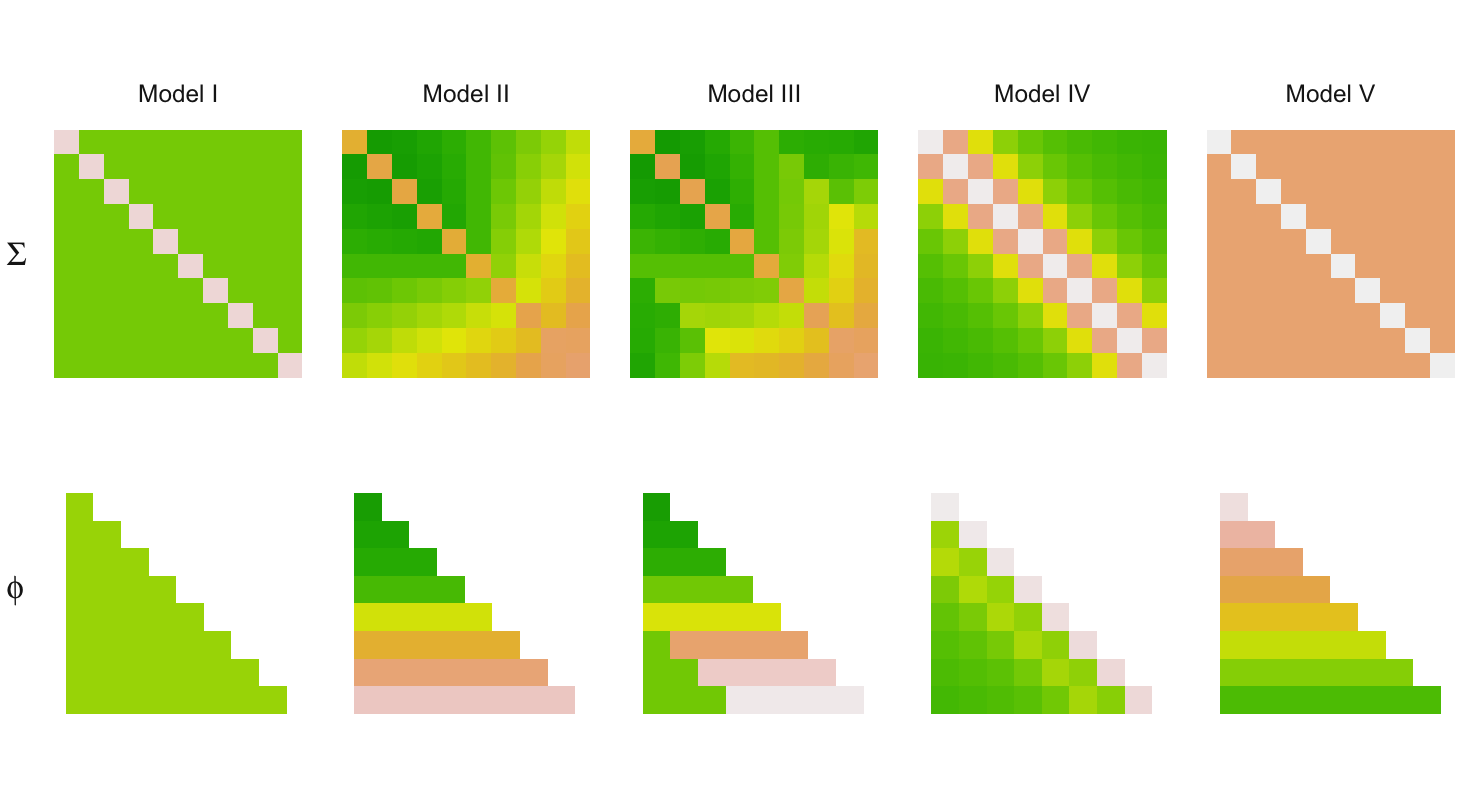
\includegraphics[width = 1.1\textwidth]{img/cov-cholesky-grid}%}
\caption{\textit{Heatmaps of the true covariance matrices corresponding to Model I - Model V and $\phi$ defining the corresponding Cholesky factor $T$. The smallest elements of each matrix correspond to dark green pixels; the light pink (white) pixels correspond to the large (largest) elements of the matrix.} } \label{fig:true-covariance-heatmaps}
\end{center}
\end{figure}

%\begin{center}
%\fbox{
\begin{description}[style=multiline, leftmargin=3cm, font=\normalfont]
\item[\textit{Model I:} ] $\Sigma = I$ (\textit{the identity matrix.})
\item[\textit{Model II:} ] $\Sigma^{-1} = T' D^{-1} T$, where $D = 0.01 \times I$, and $T = \left[-\tilde{\phi}\left(t_i, t_j\right)\right]$ with $\tilde{\phi}\left(t_i,t_i\right) = 1$,
							 $\tilde{\phi}\left(t_i,t_j\right) = t_i - \frac{1}{2}$ for $0 \le t_j < t_i \le 1$, $\tilde{\phi}\left(t_i,t_j\right) = 0$ otherwise.
\item[\textit{Model III:} ] $\Sigma^{-1} = T' D^{-1} T$, where $D = 0.01 \times I$, and $T = \left[-\tilde{\phi}\left(t_i, t_j\right)\right]$ with $\tilde{\phi}\left(t_i,t_i\right) = 1$,
							 $\tilde{\phi}\left(t_i,t_j\right) = t_i - \frac{1}{2}$ for $0 \le t_i - t_j \le \frac{1}{2}$, $\tilde{\phi}\left(t_i,t_j\right) = 0$ otherwise.
\item[\textit{Model IV:} ] $\Sigma = \left[\sigma_{ij}\right]$, $\sigma_{ij} = \left(1 + \frac{\left(t_i - t_j\right)^2}{2 k^2}\right)$ where $k = 0.6$, $0 < t_i, t_j < 1$ (\textit{the rational quadratic model}.)
\item[\textit{Model V:} ] $\Sigma = {T^{-1}}' D T^{-1} = \rho \mathrm{J} + \left(1-\rho\right)\mathrm{I}$, $\rho = 0.7$, where $D = \mbox{diag}\left(\sigma_t^2,\dots, \sigma_p^2\right)$ with $\sigma_t^2 = 1 -\frac{\left(t-2\right)\rho^2}{1 + \left(t-2\right)\rho}$, $t = 2,\dots, p$, $T = \left[-\tilde{\phi}\left(t, s\right)\right]$ with $\tilde{\phi}\left(t,t\right) = 1$, $\tilde{\phi}\left(t,s\right) = 1 -\frac{\left(t-2\right)\rho^2}{1 + \left(t-2\right)\rho}$ for $t = 2, \dots, p$, $\tilde{\phi}\left(t,s\right) = 0$ otherwise (\textit{the compound symmetry model.}) 
\end{description} %}
%\captionof{InfoBox}{Simulation data was generated according to Model I - Model V. \label{fg:sim-models}}
%\end{center}

To assess performance of an estimator $\hat{\Sigma}$, we consider the entropy loss
\begin{equation*} \label{eq:quad-loss}
\Delta\left(\Sigma,\hat{\Sigma}\right) = tr\left( \Sigma^{-1} \hat{\Sigma} \right) - \log \vert \Sigma^{-1} \hat{\Sigma} \vert - p,
\end{equation*}
\noindent
which can be derived from the Wishart likelihood \cite{Anderson84a}. Given $\Sigma$, we prefer the estimator with the smallest risk
\begin{equation*}
R \left(\Sigma,\hat{\Sigma}\right) = E_\Sigma\left[\Delta\left(\Sigma,\hat{\Sigma}\right)\right], 
\end{equation*}
\noindent
which we approximate via Monte Carlo simulation. For each combination of $p = 10, 20, 30$ and sample size $N = 50, 100$, we construct an estimate from each of $100$ samples from a mean zero $p$-dimensional multivariate Normal distribution with covariance matrix $\Sigma = T^{-1} D {T'}^{-1}$ and calculate the corresponding loss. 

Construction of the sample covariance matrix $S$ and regularized variants $S^\omega$ and $S^\lambda$ requires an equal number of observations on each subject taken at a common set of observation times, so simulations were conducted using complete data, with observation times $t = 1, \dots, p$ mapped to the unit interval. The smoothing spline estimator $\hat{\Sigma}_{SS}$ was constructed by using a tensor product cubic smoothing spline for $\phi$ and univariate cubic smoothing spline for $\sigma^2\left(t\right)$.

Figure~\ref{fig:cov-estimate-lattice} provides a visual summary of the qualitative differences between the estimates resulting from each of the eight methods of estimation for the five covariance structures used for simulation. The first row in the grid shows the surface plot of each of the true covariance structures, and each row thereafter corresponds to the five covariance estimates for the given estimation method; the oracle estimate in the second row serves as a point of reference for the `gold standard' in each simulation setting. 
\begin{figure}[H] 
\centering
  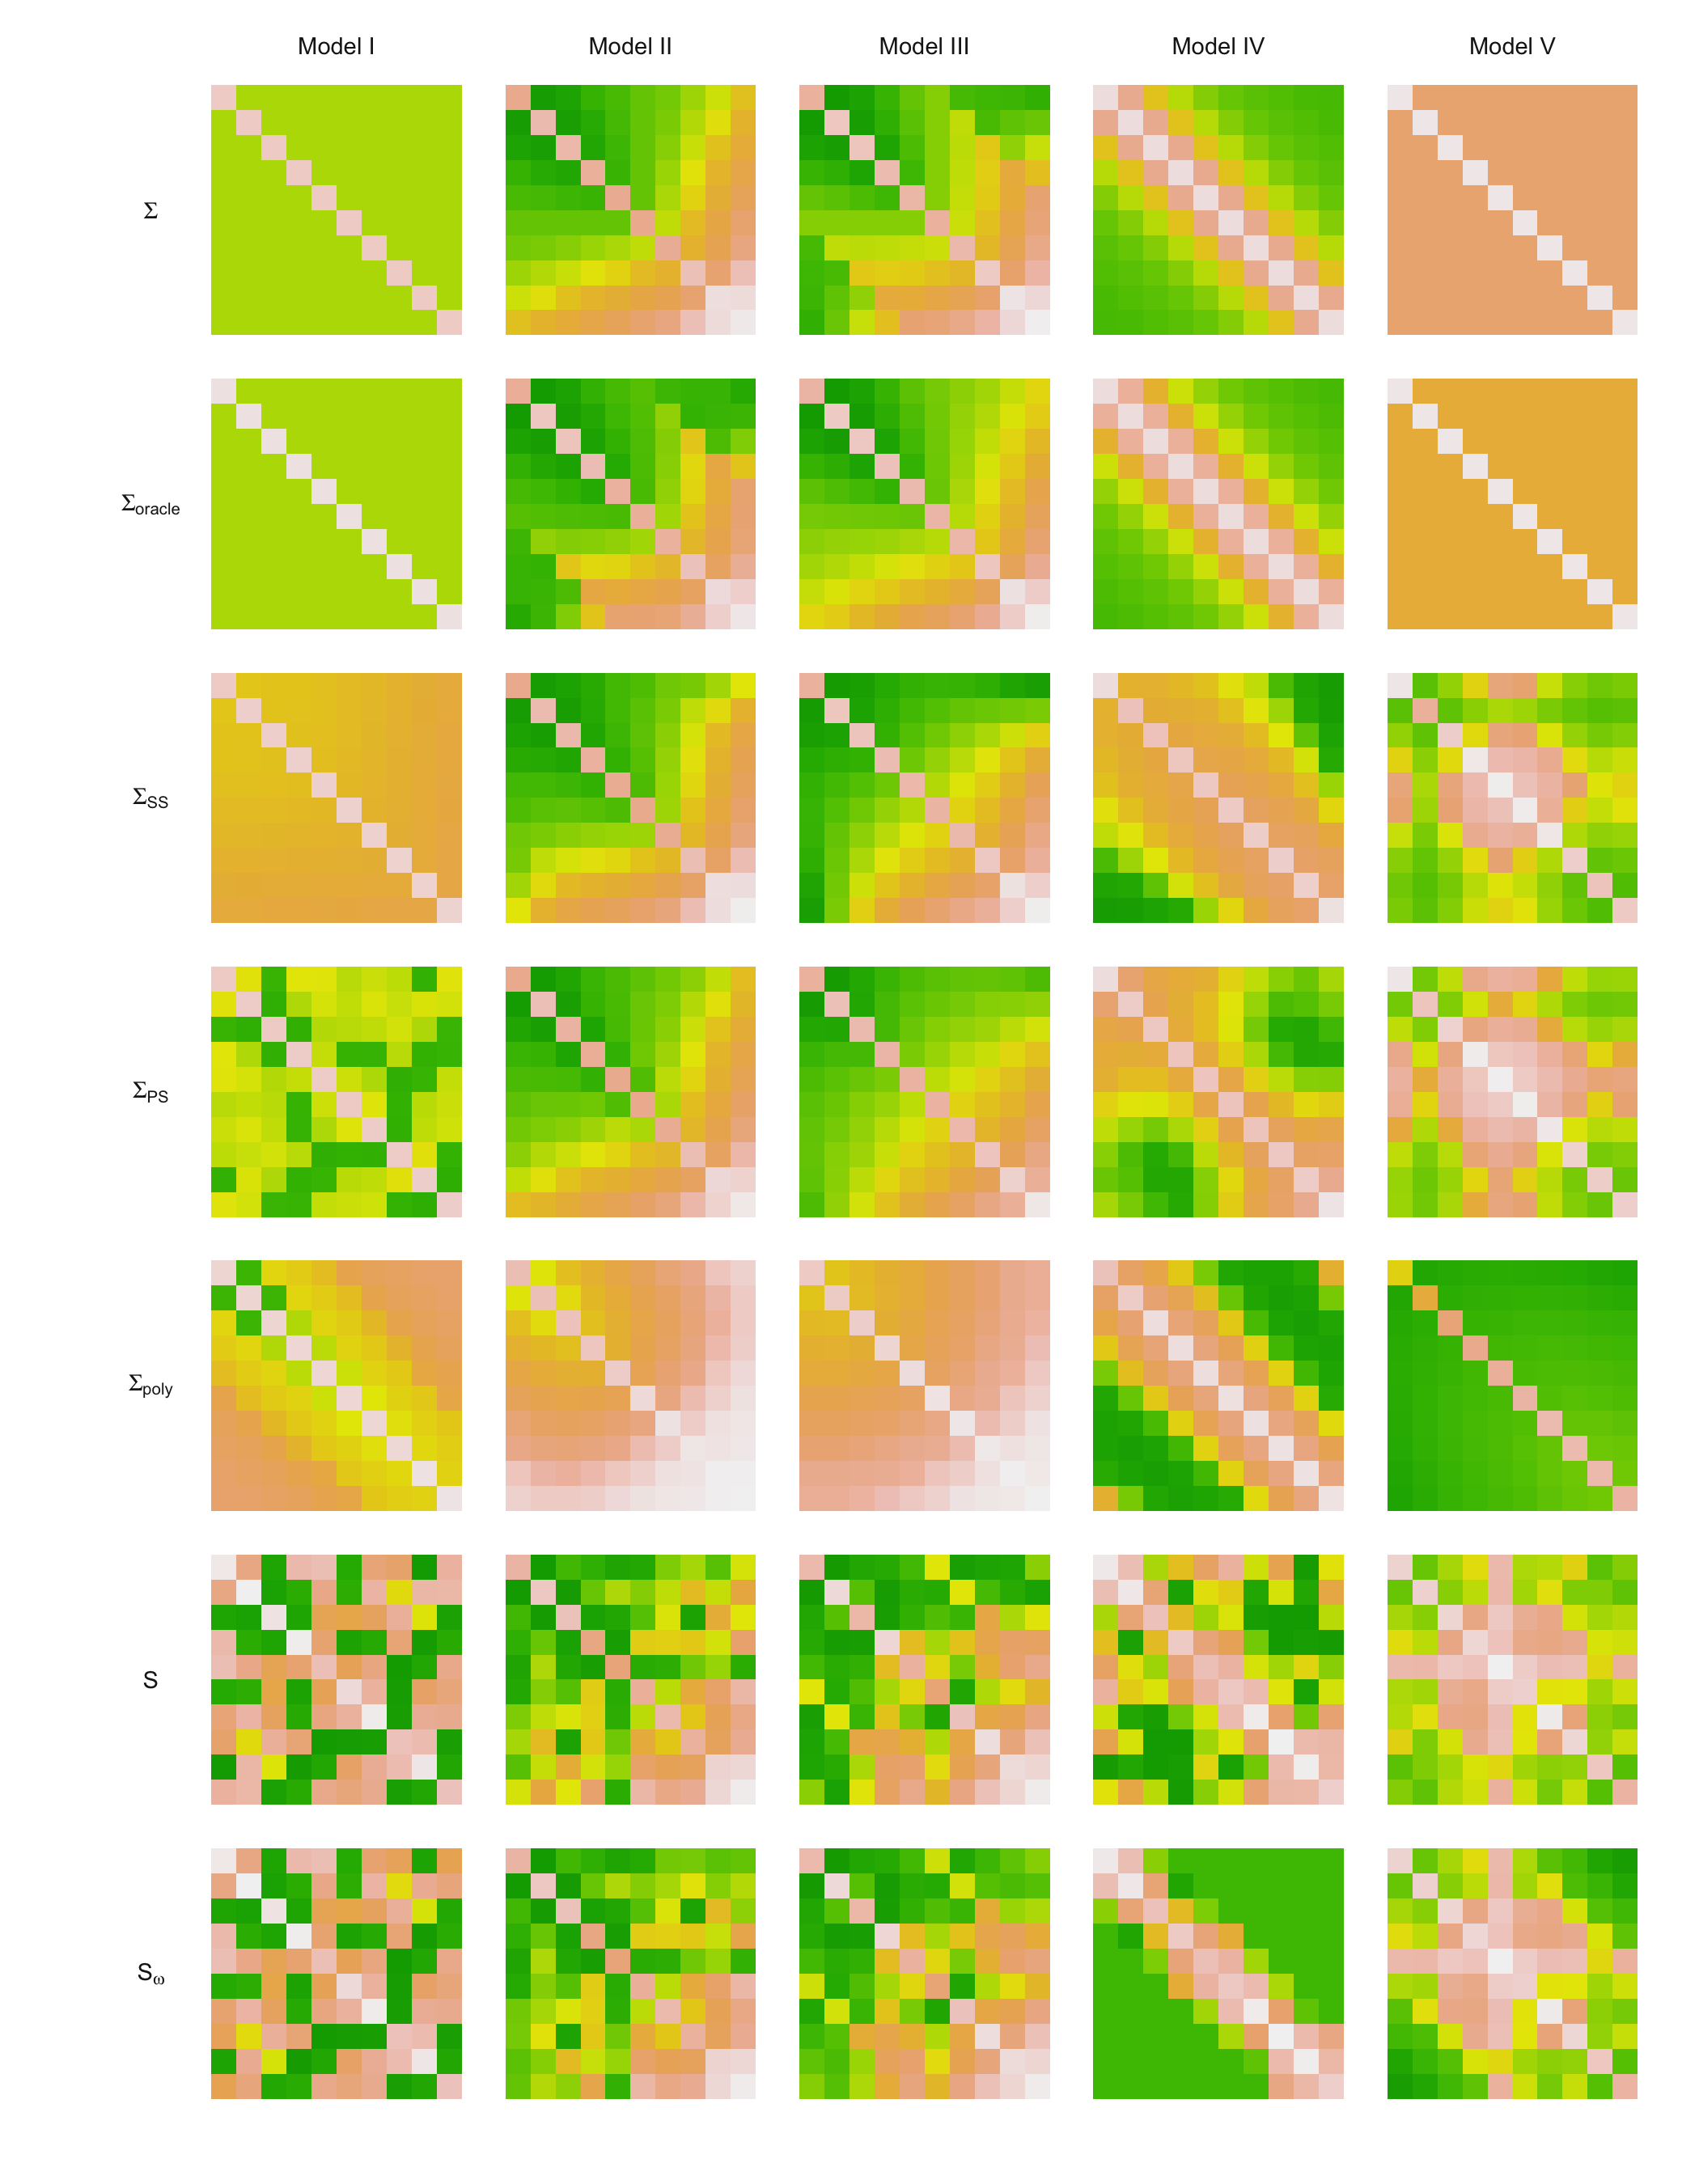
\includegraphics[width = 1\textwidth]{img/cov-estimate-lattice}
  \vspace*{-10mm}
  \caption{\textit{Covariance Model I - Model V used for simulation and corresponding estimates; true covariance structure are shown in the first row.}}\label{fig:cov-estimate-lattice}
\end{figure}
Results are presented in Table~\ref{table:simulation-1-entropy-loss}. Smoothing parameters for $\hat{\Sigma}_{SS}$ were chosen using the unbiased risk estimate \cite[Chapter ~3.22]{gu2013smoothing} and leave-one-subject-out cross validation. Performance is similar under both criteria; for brevity, results under losoCV can be found in the Appendix. For each simulation setting, the risk of the oracle estimator serves as a lower bound on the risk for the given covariance structure. 

In general, our estimator outperforms the alternative estimators, particularly when the underlying true covariance matrix does not satisfy the implicit structural assumptions motivating their construction. While the sample covariance matrix is an unbiased estimator of the unstructured covariance matrix,  the smoothing spline estimator is better for every simulation model, and the difference is larger as $p$ increases. The smoothing spline estimator performs the most poorly on Model III, where $\phi$ does not belong to the tensor product smoothing spline model space due to its discontinuous first derivative. Overall, the results indicate that the smoothing spline estimator achieves what it was designed to do; it provides a more stable estimate than the sample covariance matrix, but is guaranteed to be positive-definite unlike the soft thresholding estimator and the tapering estimator. It achieves this stability with added flexibility over the polynomial estimator. 

\setlength{\dashlinedash}{0.75pt}
\setlength{\dashlinegap}{1pt}
\setlength{\arrayrulewidth}{0.2pt}
\setlength \extrarowheight{-3pt}
\begin{small}
\begin{center}
\begin{longtable}[H]{| l | l | l | r r r r r r |}
\hline
   \hline
 \multicolumn{2}{|c}{ $$} &  \multicolumn{1}{c}{ $p$} & \multicolumn{1}{c}{$\hat{\Sigma}_{oracle}$} & \multicolumn{1}{c}{$\hat{\Sigma}_{SS}$} & \multicolumn{1}{c}{$\hat{\Sigma}_{poly}$} &
 		\multicolumn{1}{c}{$S$} & \multicolumn{1}{c}{$S^\omega$}  & \multicolumn{1}{c|}{$S^\lambda$} \\ 
\hline
   \hline
\endfirsthead
%\hline
 \multicolumn{2}{|c}{$$} &  \multicolumn{1}{c}{ $p$} & \multicolumn{1}{c}{$\hat{\Sigma}_{oracle}$} & \multicolumn{1}{c}{$\hat{\Sigma}_{SS}$} & \multicolumn{1}{c}{$\hat{\Sigma}_{poly}$} &
 		\multicolumn{1}{c}{$S$} & \multicolumn{1}{c}{$S^\omega$}  & \multicolumn{1}{c|}{$S^\lambda$} \\ 
\hline
   \hline
\endhead
\endfoot
%\hline
\endlastfoot
% \multicolumn{9}{c}{Model I} \\
      \hline
\multirow{6}{*}{Model I}& \multicolumn{1}{c|}{$N = 50$} &  \multicolumn{1}{c}{10} &0.0135 & 0.0685 &   0.1102 & 1.2047 & 0.5369 & 1.1742 \\ 
&   &  \multicolumn{1}{c}{$20$} & 0.0229 & 0.0834 &  0.1096 & 4.9850 & 1.3957 & 4.7796 \\ 
 &  &  \multicolumn{1}{c}{$30$} & 0.0196 & 0.1102 &  0.1127 & 12.5517 & 2.8019 & 11.3175 \\ 
\cdashline{2-9} 
 &\multicolumn{1}{c|}{$N = 100$} &  \multicolumn{1}{c}{$10$} & 0.0105 & 0.0451 &  0.0531 & 0.5685 & 0.2045 & 0.5236 \\ 
 &  &  \multicolumn{1}{c}{$20$} & 0.0105 &0.0425 & 0.0512 & 2.2831 & 0.5724 & 2.1358 \\ 
 &  &  \multicolumn{1}{c}{$30$} &0.0139 & 0.0431 &  0.0472 & 5.2770 & 1.2430 & 4.9126 \\ 
%\hline
%  \multicolumn{9}{c}{Model II} \\
   \hline
\multirow{6}{*}{Model II} & \multicolumn{1}{c|}{$N = 50$} &  \multicolumn{1}{c}{$10$} & 0.0581 &  0.0689 & 4.7673 & 1.2832 & 1.4644 & 1.1770 \\ 
&   &  \multicolumn{1}{c}{$20$} &0.0439 & 0.0581 &  97.2334 & 5.1665 & 21.6407 & 39.3522 \\ 
&     &  \multicolumn{1}{c}{$30$} & 0.0627 & 0.0811 &   153.9665 & 12.3582 & 55.3674 & 133.9980 \\ 
\cdashline{2-9} 
&   \multicolumn{1}{c|}{$N = 100$} &  \multicolumn{1}{c}{10} &  0.0386 & 0.0457  & 4.7911 & 0.5812 & 0.8335 & 0.5628 \\ 
&    &  \multicolumn{1}{c}{$20$} & 0.0269 & 0.0416 &   98.1989 & 2.3364 & 10.1841 & 10.0864 \\ 
&    &  \multicolumn{1}{c}{$30$} &  0.0288 & 0.0367 & 158.2480 & 5.2389 & 33.5207 & 62.5030 \\
       \hline
%    \multicolumn{9}{c}{Model III} \\
%   \hline
\multirow{6}{*}{Model III} & \multicolumn{1}{c|}{$N = 50$} &  \multicolumn{1}{c}{10} & 0.0619 & 0.3296 & 3.0108 & 1.2030 & 1.1460 & 1.1467 \\ 
  &    &  \multicolumn{1}{c}{$20$} &0.0695 & 1.1100  &  62.7522 & 4.9824 & 17.2244 & 14.9189 \\ 
  &  &  \multicolumn{1}{c}{$30$} &0.0576 & 2.3215 &   1091.1933 & 12.4792 & 49.9135 & 121.7795 \\ 
  \cdashline{2-9} 
&      \multicolumn{1}{c|}{$N = 100$} &  \multicolumn{1}{c}{$10$} & 0.0268 &  0.2904 & 3.0383 & 0.5699 & 0.5545 & 0.5371 \\ 
&     &  \multicolumn{1}{c}{$20$} & 0.0275 & 1.1963 & 62.8960 & 2.2700 & 11.8274 & 9.5217 \\ 
&    &  \multicolumn{1}{c}{$30$} &  0.0221 & 2.2811 & 1105.0449 & 5.2234 & 29.1693 & 60.3529 \\ 
       \hline
  %    \multicolumn{9}{c}{Model IV} \\
  % \hline
\multirow{6}{*}{Model IV} & \multicolumn{1}{c|}{$N = 50$} & \multicolumn{1}{c}{$10$} & 0.0217 & 0.3348 & 0.7144 & 1.2218 & 0.7397 & 1.1921 \\ 
&  &  \multicolumn{1}{c}{$20$} &0.0286 & 0.9177 &  1.4588 & 4.9091 & 1.9786 & 4.9206 \\ 
&      &  \multicolumn{1}{c}{$30$} &  0.0283 &1.5992  & 2.2173 & 12.6114 & 3.7440 & 12.1489 \\ 
\cdashline{2-9} 
 &  \multicolumn{1}{c|}{$N = 100$} & \multicolumn{1}{c}{10} & 0.0125 & 0.3047 &  0.6958 & 0.5570 & 0.3168 & 0.5515 \\ 
&      &  \multicolumn{1}{c}{$20$} &0.0105 & 0.8911  &  1.4813 & 2.2659 & 0.9365 & 2.2474 \\ 
 &     &  \multicolumn{1}{c}{$30$} & 0.0134 & 1.5213 & 2.2228 & 5.2106 & 1.9312 & 5.2111 \\ 
       \hline
%      \multicolumn{9}{c}{Model V} \\
%   \hline
\multirow{6}{*}{Model V}  & \multicolumn{1}{c|}{$N = 50$} &  \multicolumn{1}{c}{$10$} & 0.0986 &0.2769 & 1.2420 & 1.2023 & 18.5222 & 2.9824 \\ 
&  &  \multicolumn{1}{c}{$20$} &0.2512 & 0.7514 &   2.8557 & 5.0195 & 34.6618 & 13.8690 \\ 
&  &  \multicolumn{1}{c}{$30$} &  0.2641& 1.1776   & 4.5791 & 12.3460 & 46.5437 & 26.1364 \\ 
\cdashline{2-9} 
&  \multicolumn{1}{c|}{$N = 100$} & \multicolumn{1}{c}{10} &0.0520 & 0.2416 &   1.1491 & 0.5821 & 16.4081 & 1.7397 \\ 
&&  \multicolumn{1}{c}{$20$} & 0.0827 & 0.7286 &   2.9080 & 2.2918 & 32.5295 & 5.4649 \\ 
&  &  \multicolumn{1}{c}{$30$} &  0.1799 & 1.1813  & 4.4402 & 5.2197 & 39.2914 & 15.4295  \\
\hline
\caption{\textit{Multivariate normal simulations for Model I - Model V. Estimated entropy risk is reported for the oracle estimator, our smoothing spline ANOVA estimator, the parametric polynomial estimator of Pan and MacKenzie (2003), the sample covariance matrix, the tapered sample covariance matrix, and the soft thresholding estimator.}}
\label{table:simulation-1-entropy-loss}
\end{longtable}
\end{center}
\end{small}
\section*{\sffamily \Large DATA ANALYSIS}
\cite{kenward1987method} reported an experiment designed to investigate the impact of the control of intestinal parasites in cattle. To compare two methods for controlling the disease, say treatment A and treatment B, each of 60 cattle were assigned randomly to two groups, each of size 30. Animal subjects were put out to pasture at the start of grazing season, with each member of the groups receiving one of the two treatments. Animals were weighed $p = 11$ times over a 133-day period; the first 10 measurements on each animal were made at two-week intervals and the final measurement was made one week later. The longitudinal dataset is balanced, as there were no missing observations for any of the experimental units. Observed weights are shown in Figure~\ref{fig:cattle-weights-by-trt}.
\begin{center}  
\begin{figure}[H] 
\begin{center}
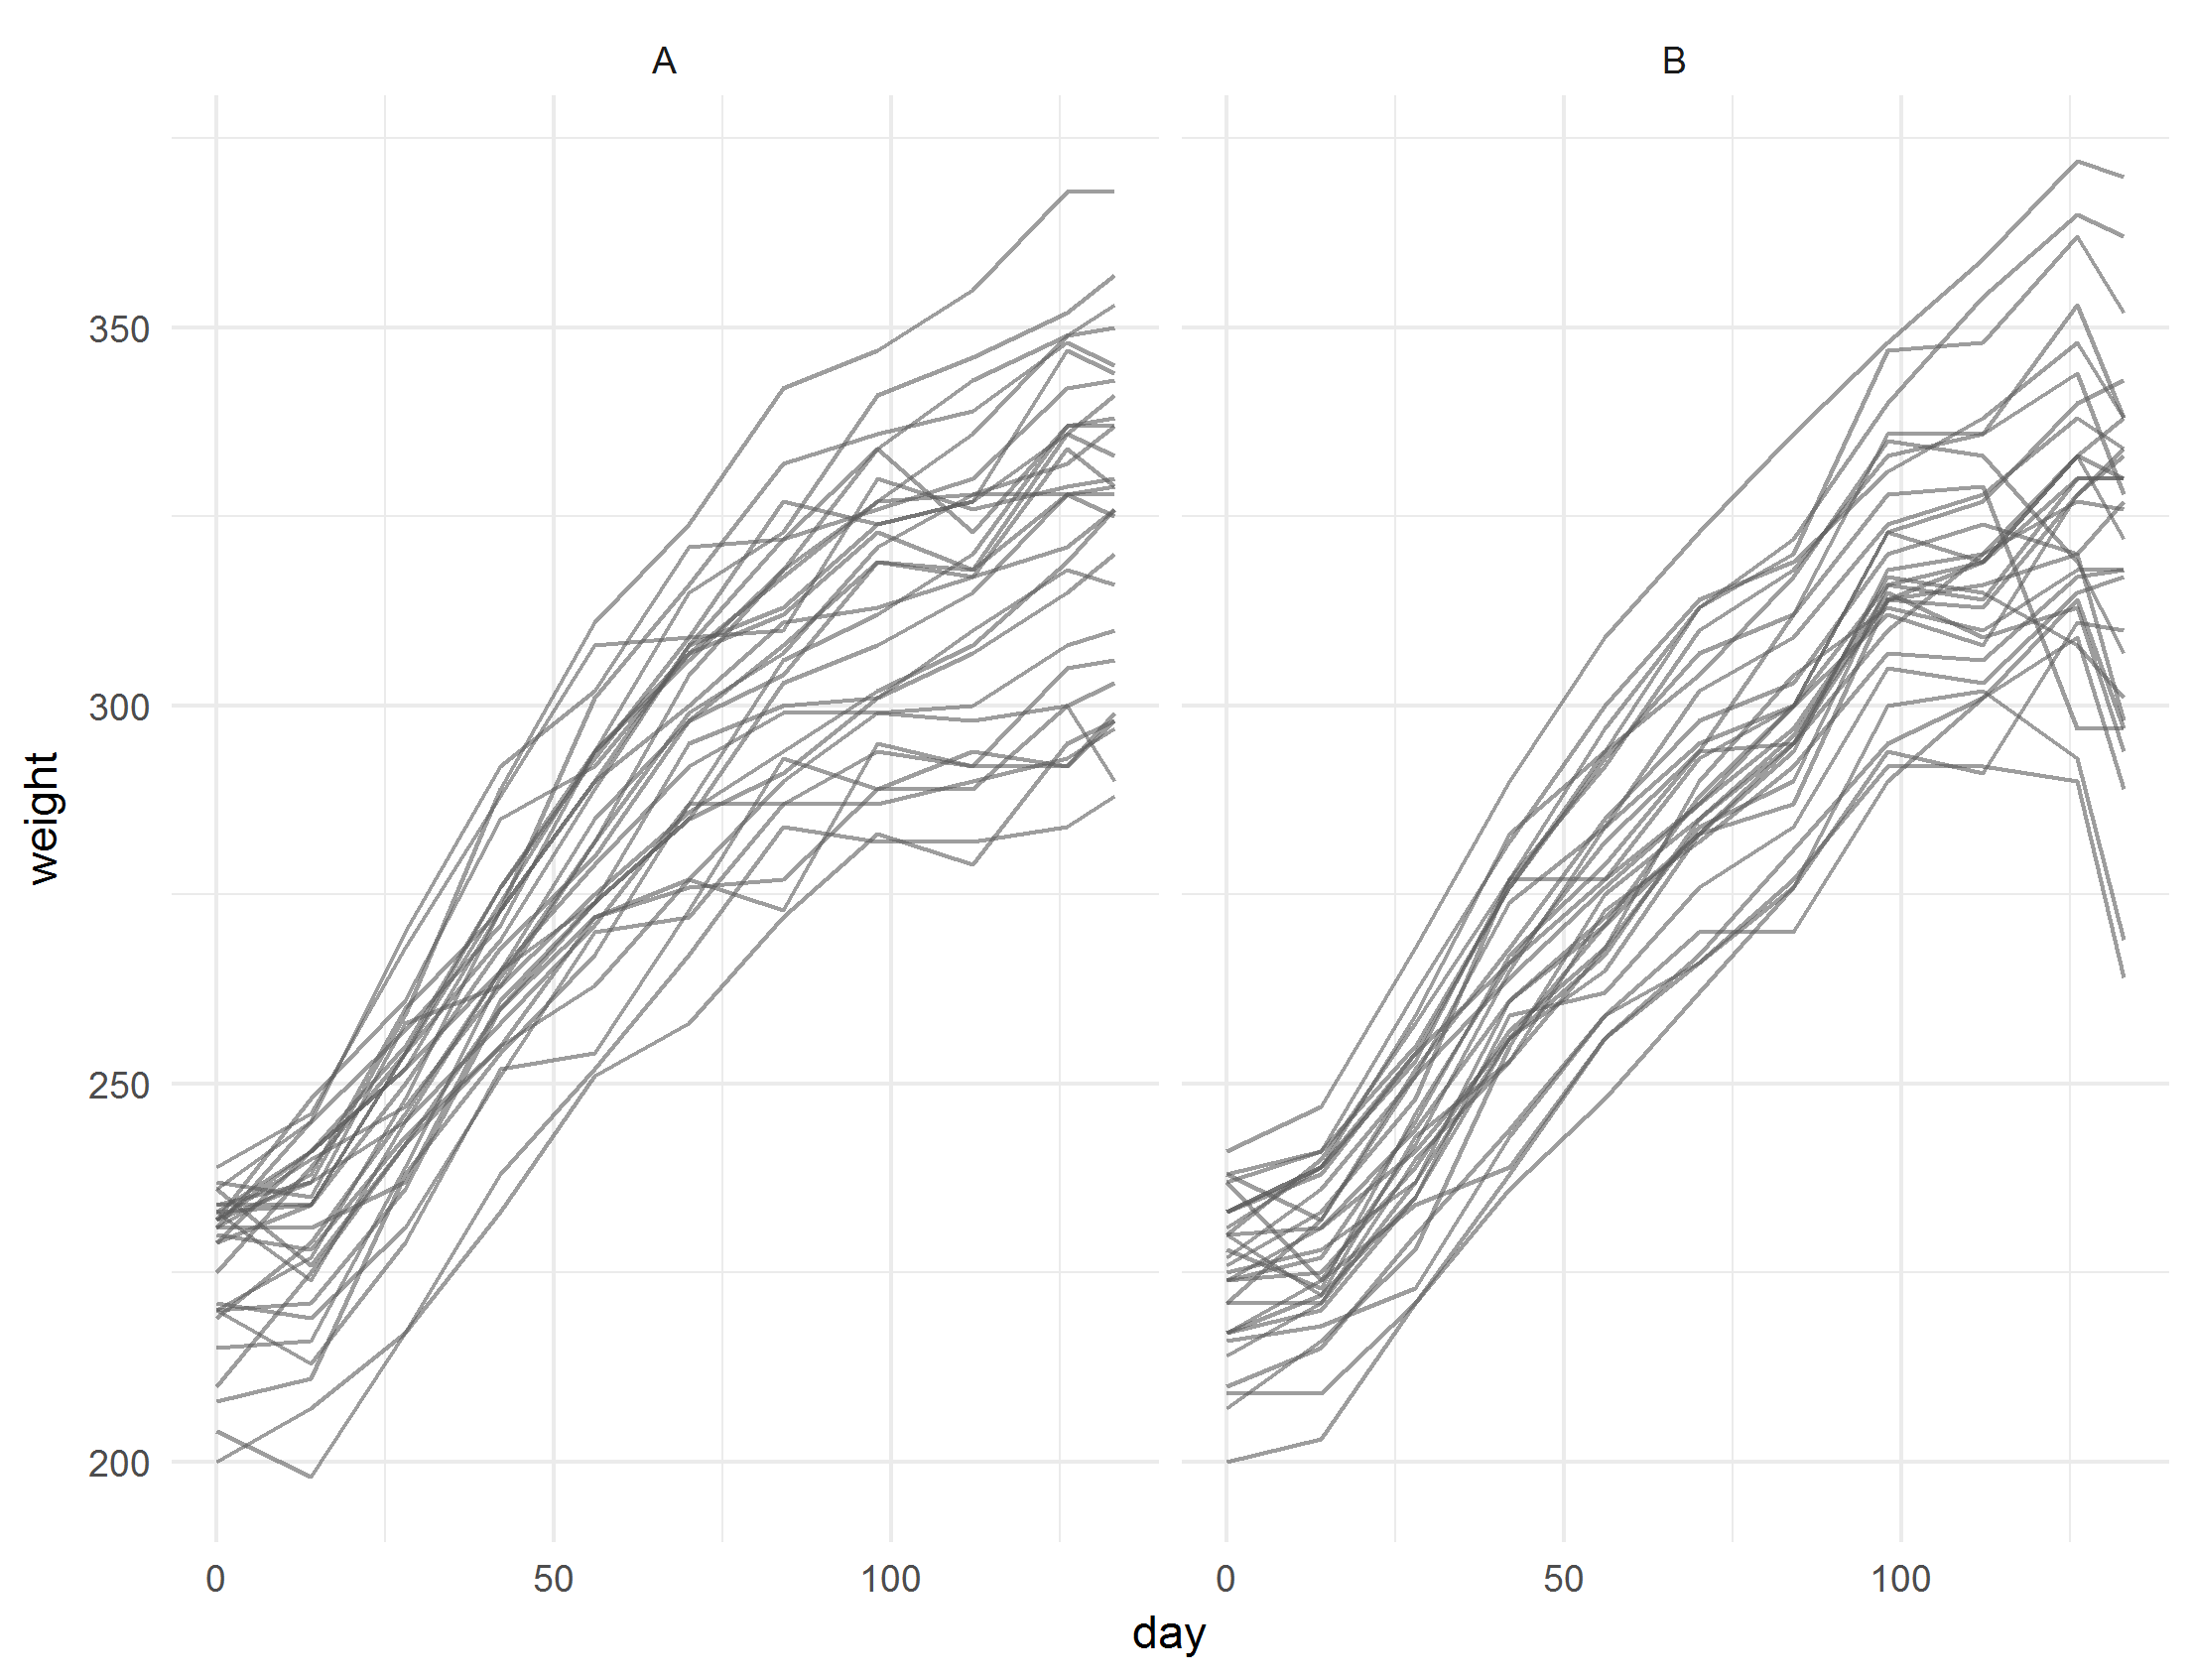
\includegraphics[width = .8\textwidth, height = 3.5in]{img/cattle-weights-vs-time-by-trt}
\caption{\textit{Subject-specific weight curves over time for treatment groups A and B.}}\label{fig:cattle-weights-by-trt}
\end{center}
\end{figure} 
\end{center}
The analysis of the same dataset provided by \cite{zimmerman1997structured} rejected equality of the two covariance matrices corresponding to treatment group using the classical likelihood ratio test, making it reasonable to study each treatment group's covariance matrix separately. Following \cite{pan2017jmcm}, \cite{zhang2015joint}, and \cite{pourahmadi1999joint}, we analyze the data from the $N = 30$ cattle assigned to treatment group A, which we assume share a common $11 \times 11$ covariance matrix $\Sigma$. The left profile plot in Figure~\ref{fig:cattle-weights-by-trt} of the weights for units in treatment group A shows a clear upward trend in weights;  variances appear to increase over time, suggesting that the covariance structure is nonstationary.

The nonstationarity suggested in Figure~\ref{fig:cattle-weights-by-trt} is also supported by the sample correlations given in Table~\ref{table:cattleA-sample-correlations}; correlations within the subdiagonals are not constant and increase over time, a secondary indication that a stationary covariance is not appropriate for the data. 
\begin{table}[H] 
\begin{footnotesize}
\begin{center}
\begin{tabular}{r|rrrrrrrrrrr}
& \multicolumn{11}{c}{day}\\
&&&&&&&&&&\\
& 0 & 14 & 28 & 42 & 56 & 70 & 84 & 98& 112& 126 &133\\
  \hline\noalign{\smallskip} 
0 & 1.00  \\ 
  14 & 0.82 & 1.00  \\ 
  28 & 0.76 & 0.91 & 1.00 & \\ 
  42 & 0.65 & 0.86 & 0.93 & 1.00 &  \\ 
  56 & 0.63 & 0.83 & 0.89 & 0.93 & 1.00 &  \\ 
  70 & 0.58 & 0.75 & 0.85 & 0.90 & 0.94 & 1.00 & \\ 
  84 & 0.51 & 0.64 & 0.75 & 0.80 & 0.85 & 0.92 & 1.00 &\\ 
  98 & 0.52 & 0.68 & 0.77 & 0.82 & 0.88 & 0.93 & 0.92 & 1.00 & \\ 
  112 & 0.51 & 0.61 & 0.71 & 0.74 & 0.81 & 0.89 & 0.92 & 0.96 & 1.00 & \\ 
  120 & 0.46 & 0.59 & 0.69 & 0.70 & 0.77 & 0.85 & 0.86 & 0.94 & 0.96 & 1.00 &  \\ 
  133 & 0.46 & 0.56 & 0.67 & 0.67 & 0.74 & 0.81 & 0.84 & 0.91 & 0.95 & 0.98 & 1.00 \\ 
   \hline
\end{tabular}
\caption{\textit{Cattle data: treatment group A sample correlations.}}\label{table:cattleA-sample-correlations}
\end{center}
\end{footnotesize}
\end{table}
Analyzing the sample regressogram and sample innovation variogram, \cite{pourahmadi1999joint} suggested that both sample generalized autoregressive parameters and the logarithms of the innovation variances can be characterized in terms of cubic functions of the lag only. They model 
\begin{align}
\begin{split} \label{eq:pourahmadi-cubic-model}
\phi_{ts} = x'_{ts}\beta, \\
\log\left(\sigma_t^2\right) = z'_{t}\gamma, 
\end{split}
\end{align}
\noindent
for $t = t_2,\dots, t_{11}$ where 
\begin{align*}
x'_{ts} = \begin{bmatrix} 1 & t - s& \left(t - s\right)^2 & \left(t - s\right)^3 \end{bmatrix},\; \mbox{and } z'_{t} = \begin{bmatrix} 1 & t& t^2& t^3 \end{bmatrix}.
\end{align*}
\noindent
They estimate $\beta$ and $\gamma$ via maximum likelihood.  Figure~\ref{fig:cattleA-smoothed-regressogram-variogram} shows the estimated cubic polynomials corresponding to Model~\eqref{eq:pourahmadi-cubic-model}.  
 \begin{figure}[H]
\begin{center}
  \subfloat[\textit{Sample generalized autoregressive parameters $\hat{\phi}_{ts}$.}] {\label{fig:cattleA-regressogram-with-cubic-smooth} 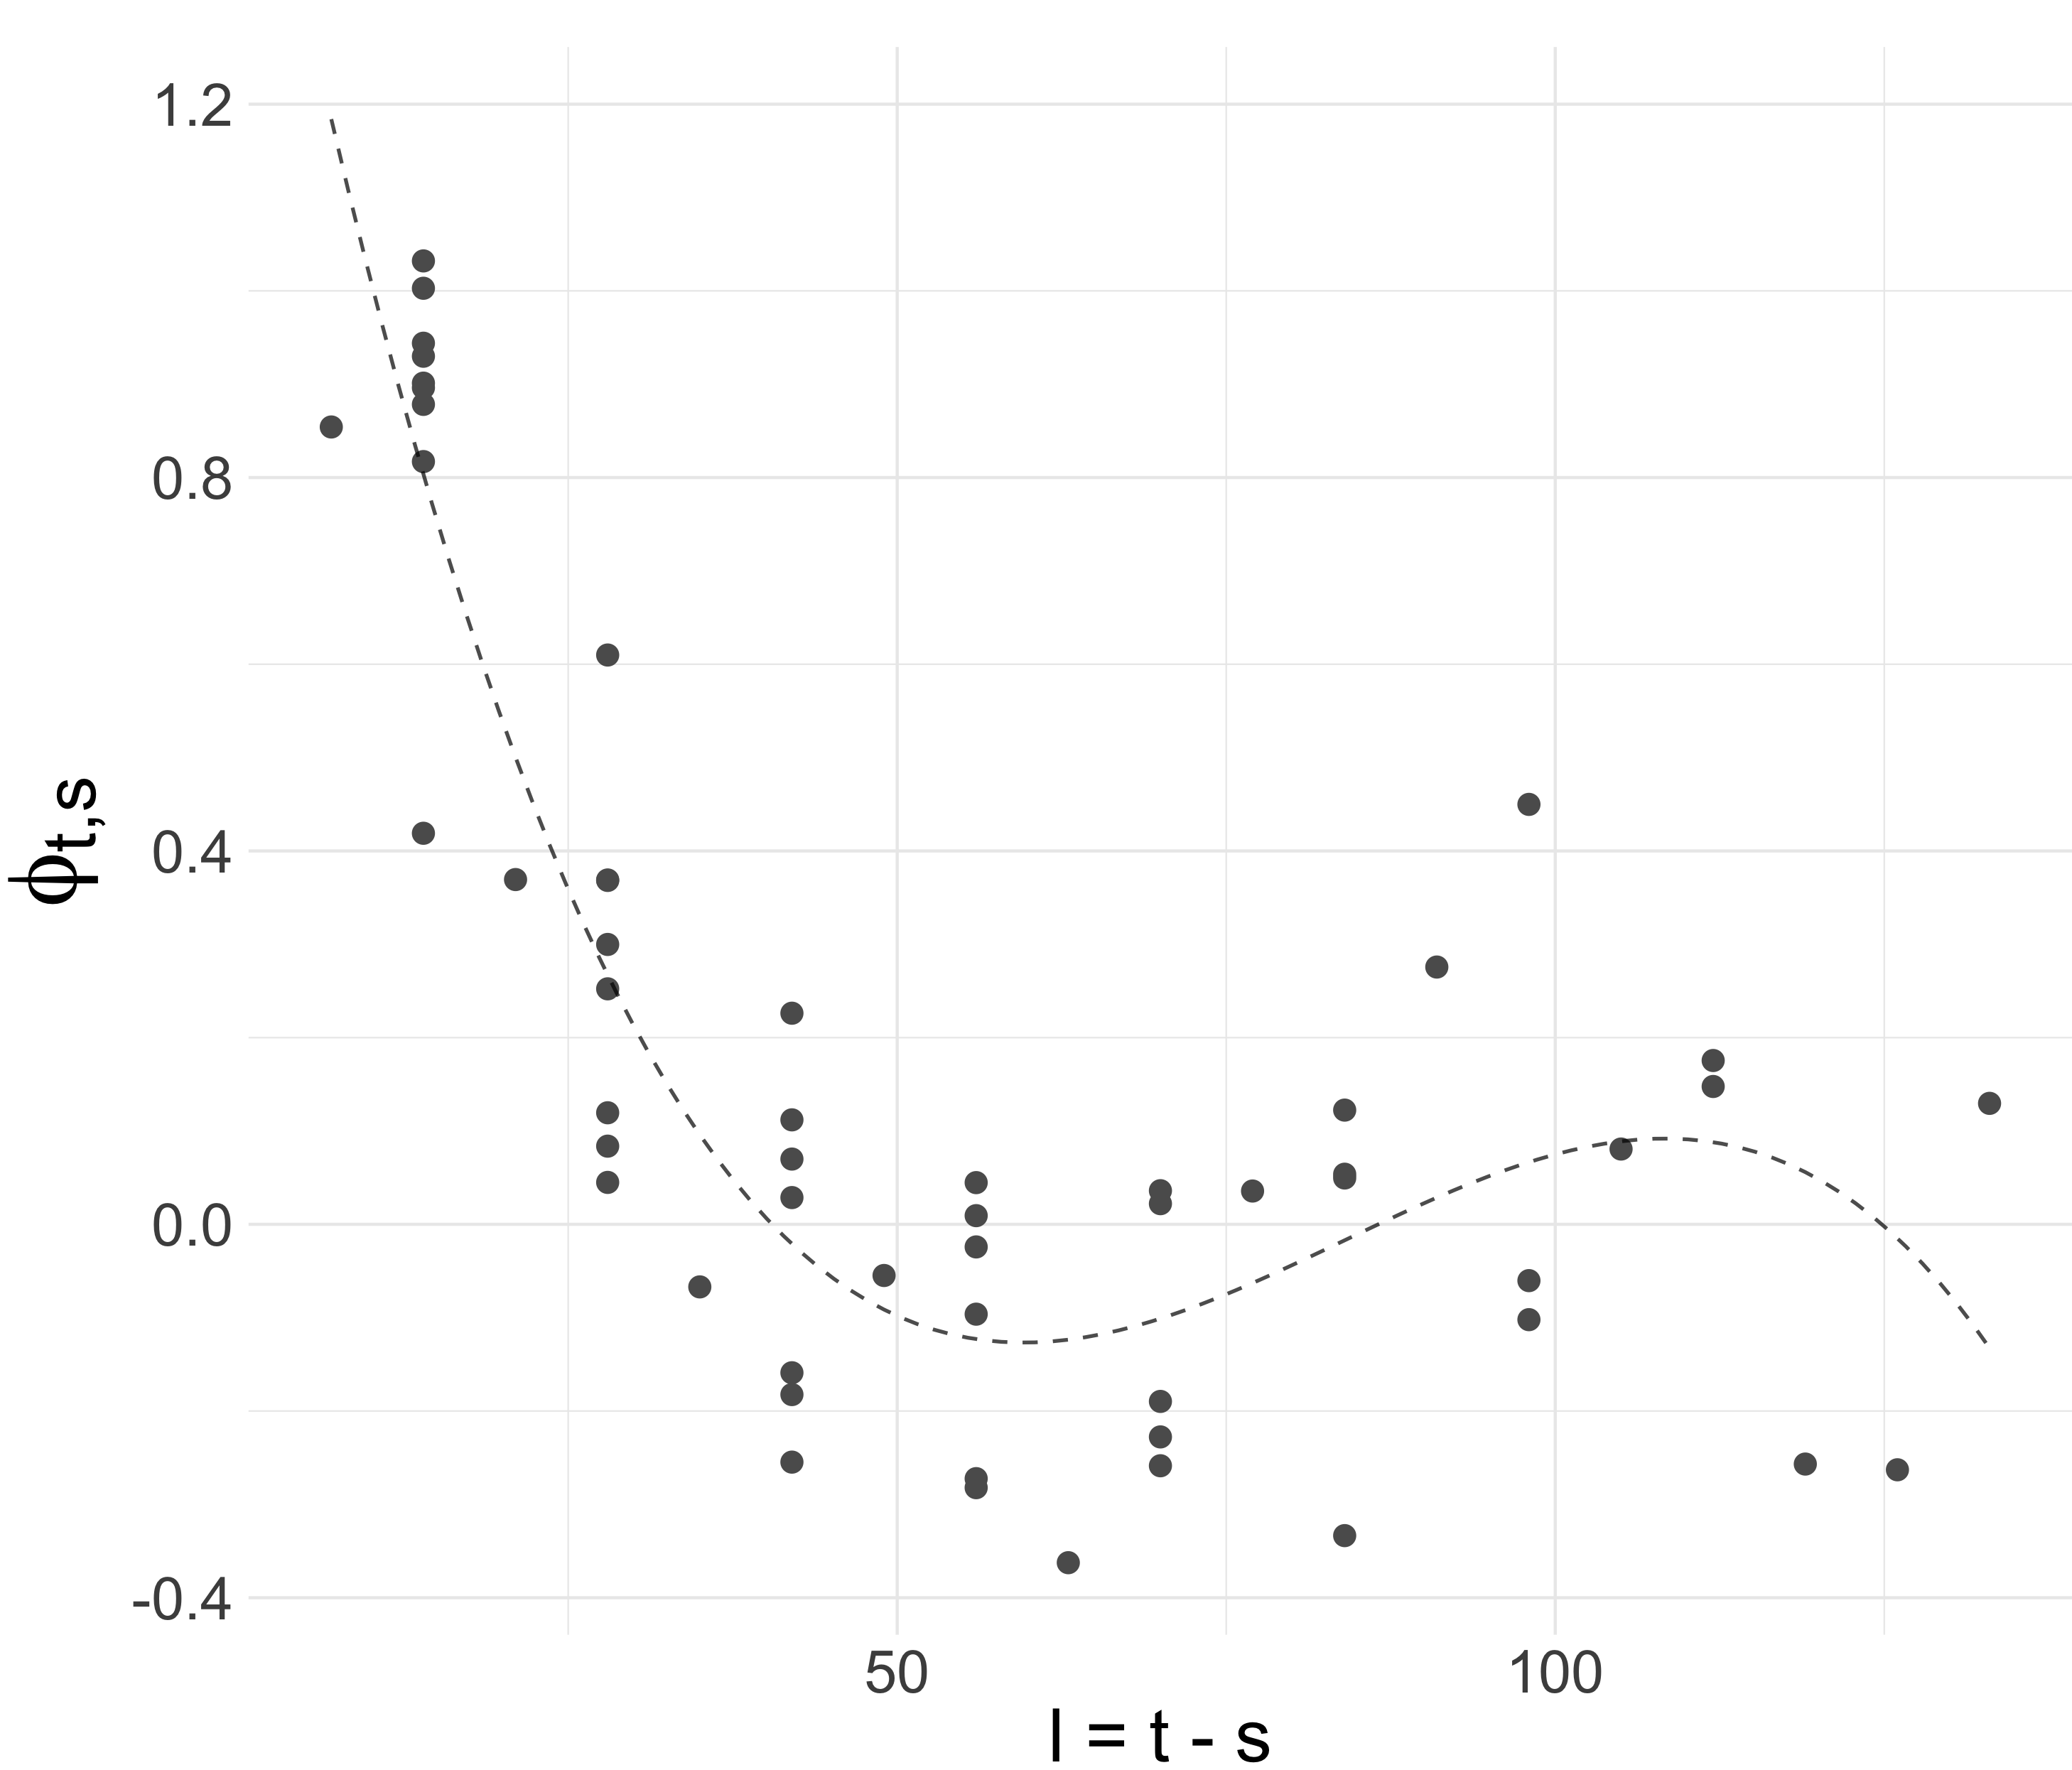
\includegraphics[width=0.45\textwidth]{img/cattleA-regressogram-with-cubic-smooth}}%\caption{\textit{Smoothed sample regressogram.}}
  \hfill
    \subfloat[\textit{Sample log innovation variances.}]{\label{fig:cattleA-innovariogram-with-cubic-smooth} 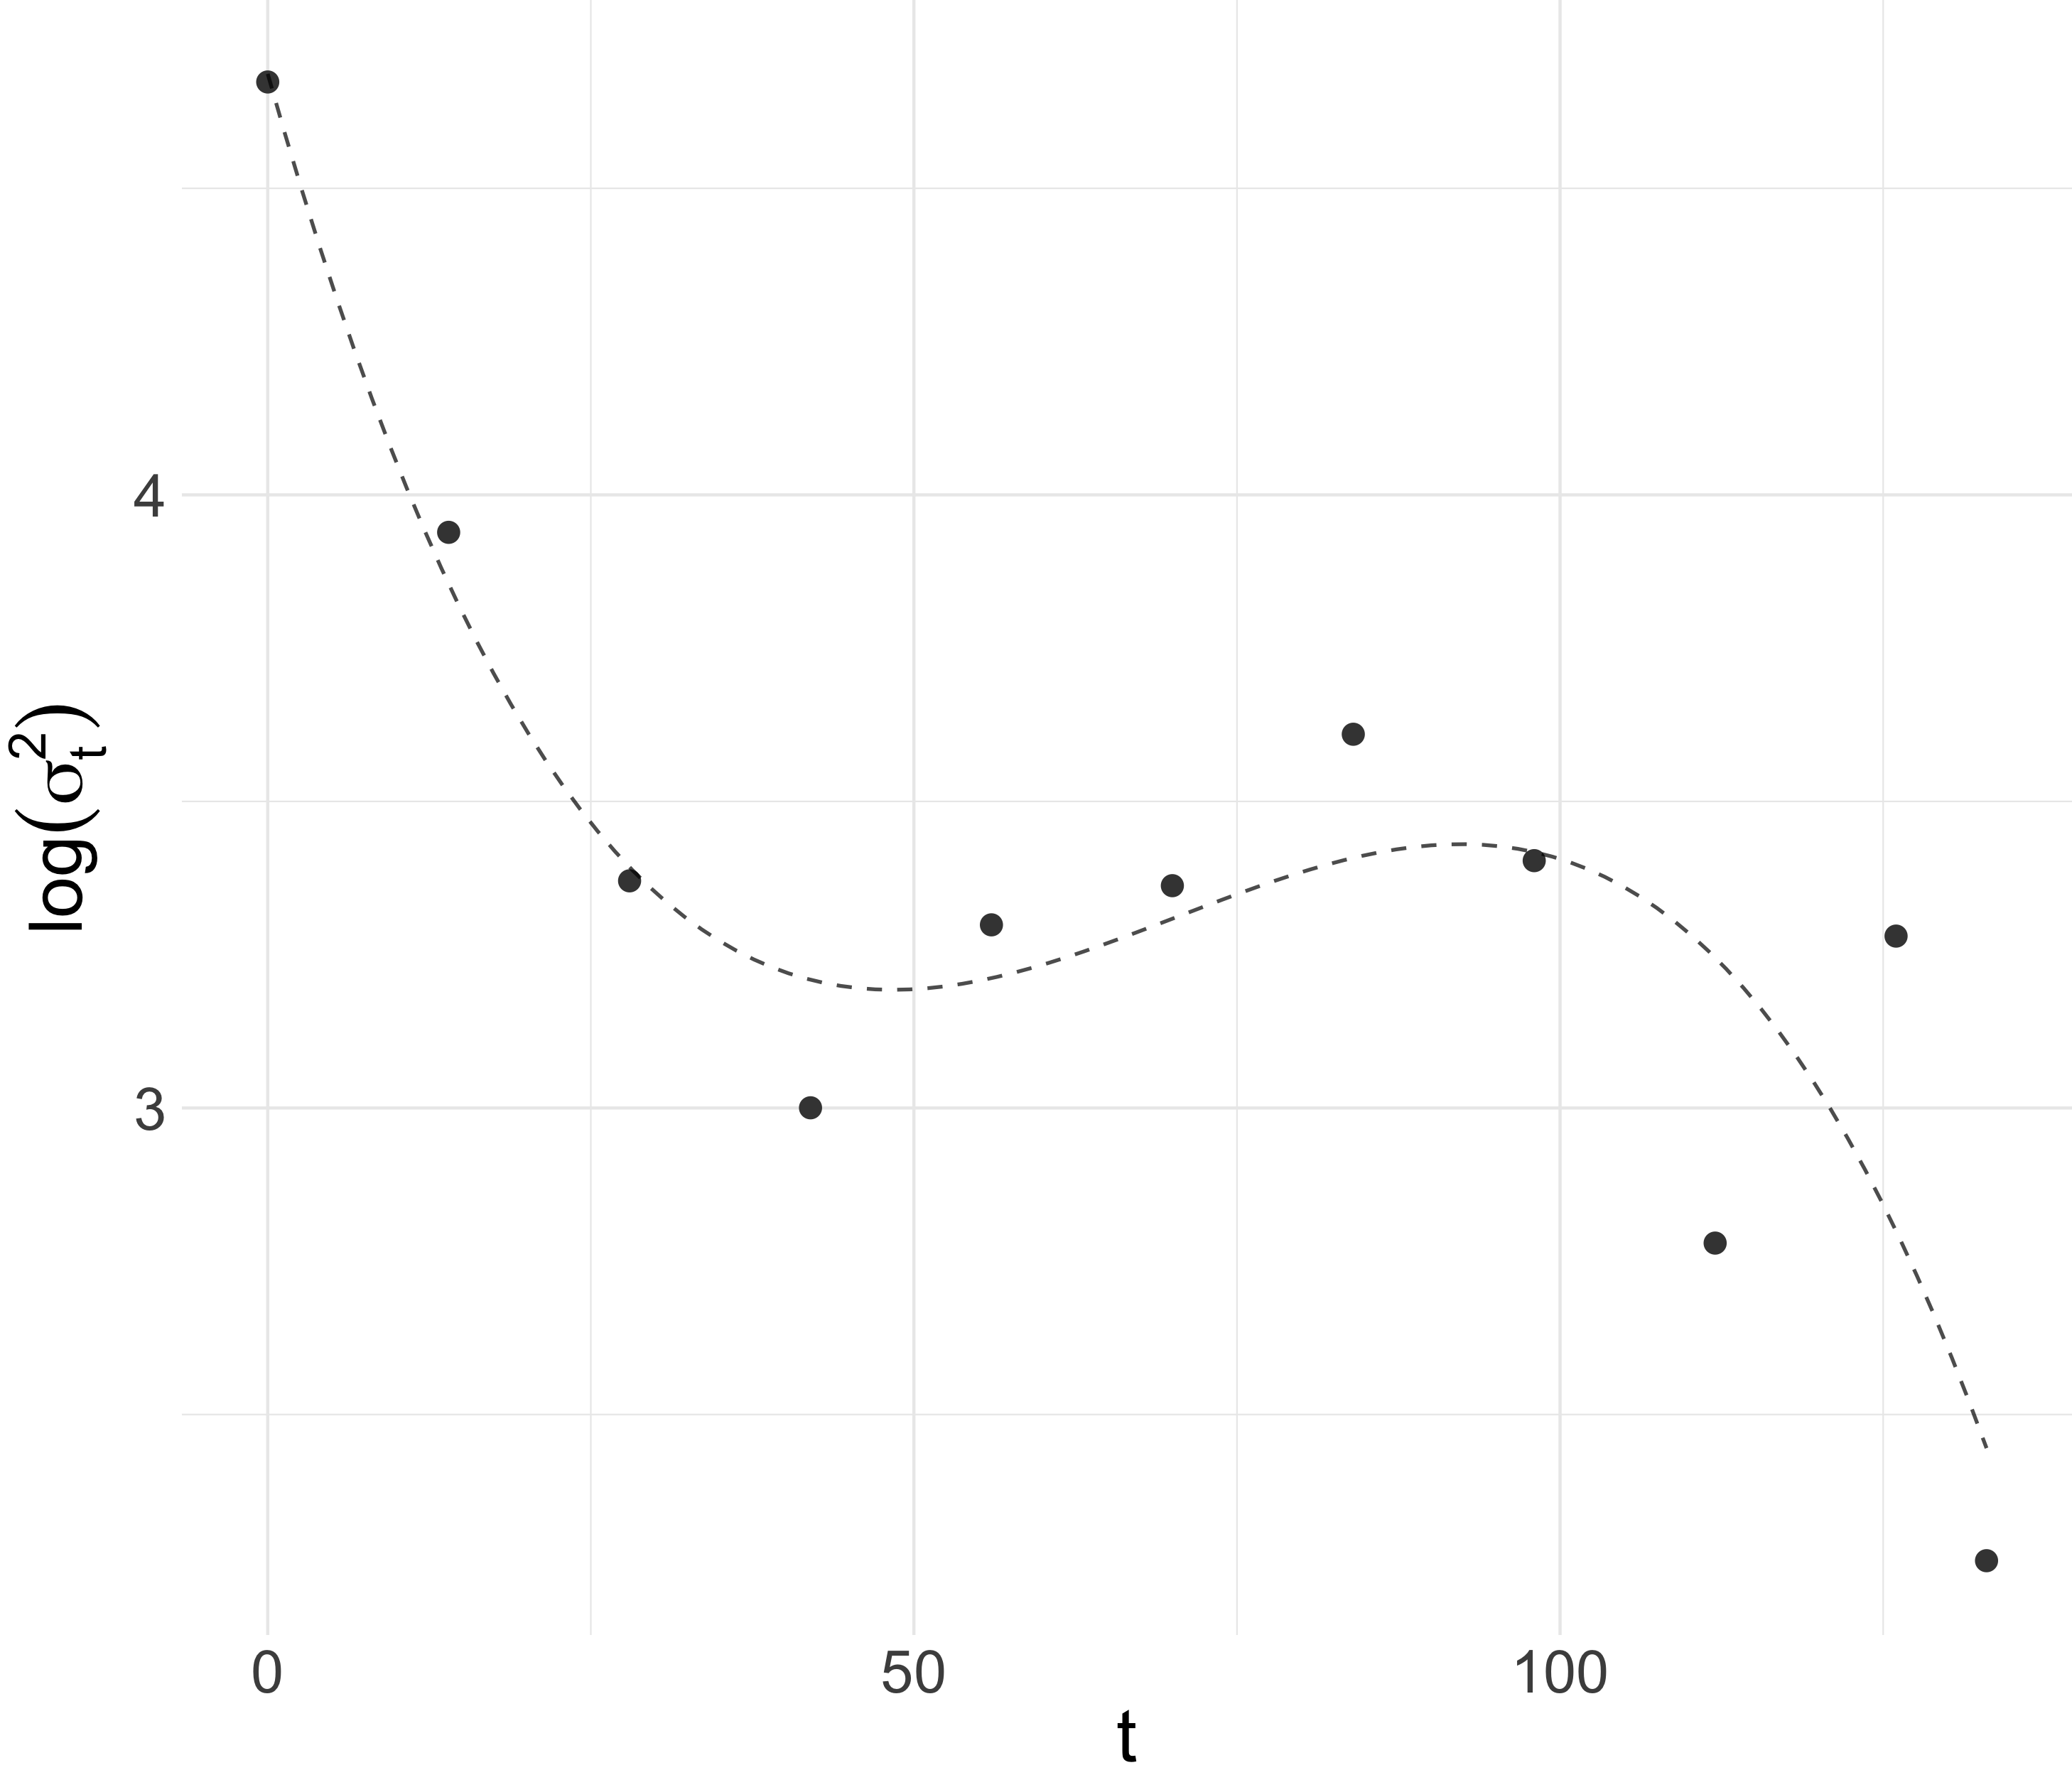
\includegraphics[width=0.45\textwidth]{img/cattleA-innovariogram-with-cubic-smooth}}%\caption{\textit{Smoothed sample log innovation variances.}}
 \caption{\textit{Cubic polynomomials fitted to the sample regressogram and log innovation variances for the cattle data from treatment group A.}} \label{fig:cattleA-smoothed-regressogram-variogram}
 \end{center}
\end{figure}
To model the mean weight trajectories, we adopt an approach akin to the dynamical conditionally linear mixed model presented in \cite{pourahmadi2002dynamic}:
\begin{equation}
Y_i = f\left(t_i  \right) + Z_i b_i + \epsilon^*_i, \quad i = 1, \dots, N,
\end{equation} 
\noindent
where $Y_i$ is the measurement corresponding response vector for the $i^{th}$ subject, $b_i$ is a $q \times 1$ vector of unknown random effects parameters, and $Z_i$ is a known $p_i \times q$ design matrix.  $f$ is the smooth function of $t$, and $t_i = \left(t_{i1}, \dots, t_{i,p_i}\right)'$ is the $p_i \times 1$ vector of measurement times for subject $i$. We take $Z_i = \left(1 , \dots, 1\right)'$ so that the random effects $\alpha_i$ correspond to subject-specific shifts. We assume to that the random intercepts are independent and identically distributed $N\left(0,\sigma_\alpha^2\right)$. We assume that the $p_i \times 1$ vector of residuals $\epsilon^*_i \sim N\left(0, \Sigma_i\right)$ are mutually independent of the random intercepts $\alpha_i$. Given that the animals belong to the same treatment group and share a common set of observation times, we assume each subject shares common covariance matrix $\Sigma_i = \Sigma$. We take the cubic smoothing spline  $f \in \hilbert = \mathcal{C}^2 = \left\{f: \; f,\;f' \mbox{ absolutely continuous, } \int\left(f''\left(x\right)\right)^2 \;dx < \infty  \right\}$, equipped with the inner product which corresponds to $J\left(f\right) = \int \left(f''\left(x\right)\right)^2\;dx$. We take the estimators of $f$, $\alpha = \left(\alpha_1,\dots, \alpha_N\right)'$ to minimize the penalized joint log likelihood
\begin{equation}
\sum_{i = 1}^N \sum_{i = 1}^{p_i} \left(y_{ij} - f\left(t_{ij} \right) - \alpha_i \right)^2 + \alpha' \Sigma_\alpha^{-1} \alpha + \lambda J \left(f\right),
\end{equation}
\noindent
where $\Sigma_\alpha = \sigma_\alpha^2 \mathrm{I}$. 

\cite{pan2017jmcm} concluded that the regressogram of empirical estimates of $\tilde{\phi}_{t,s}$ show consistent behaviour over $l = t - s$ for each value of $t$, indicating a lack of a strong functional component of $m$. This is consistent Pourahmadi's choice \cite<see>{wu2003nonparametric} in the specification of model (\ref{eq:pourahmadi-cubic-model}) in terms of lag only. To balance the consideration of previous analyses with the interest of entirely data-driven model specification, we let $\phi \in \hilbert = \hilbert_{\left[l\right]} \otimes \hilbert_{\left[m\right]}$, where 
\begin{align*} 
\hilbert_{\left[l\right]} &= \bigg\{ \phi: \phi' = 0 \bigg\} \oplus \left\{\phi: \phi\left(0\right) = {\phi'}\left(0\right) = 0; \;\; \int {\phi}''\left(l\right)\;dl < \infty   \right\} \\
\hilbert_{\left[m\right]} &= \bigg\{ \phi: \phi \propto 1 \bigg\} \oplus \left\{ \phi: \int_0^1 \phi\left(m\right) \;dm = 0, \;\; \int {\phi}''\left(m\right)\;dm < \infty \right\} 
\end{align*} %This decomposition leads to a null space comprised of functions of $l$ only, which is attractive because it coincides with the modeling assumptions made by \cite{pan2017jmcm}, \cite{huang2006covariance}, and  for the same data set.  
Figure~\ref{fig:fitted-cholesky-decomposition-cattle-date} shows the estimated Cholesky surface and innovation variance function evaluated at $t =  0,14, 28,\dots,112, 126,133$ and the corresponding pairs of observation times $\left(t,s\right)$, $0 \le s < t \le 133$. The decomposition of $\hat{\phi}$ into the functional components of its ANOVA decomposition is shown in Figure~\ref{fig:cattle-fitted-cholesky-ssanova}.
\begin{figure}[H]
\centering
    \subfloat[\textit{ $\hat{\Sigma} = \hat{T}^{-1} \hat{D} \hat{T}'^{-1} $}]{\label{fig:fitted-cholesky-decomposition-cattle-date-Sigma} 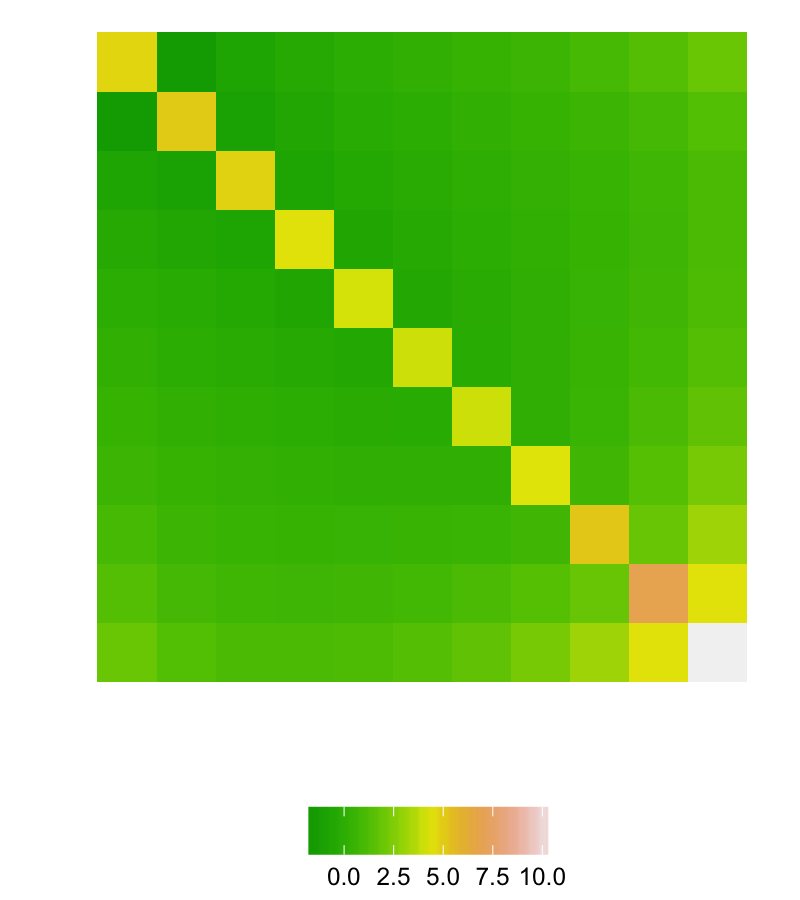
\includegraphics[width=0.25\textwidth]{img/cattle-cholesky-estimate-ggplot-Sigma}} 
  \subfloat[\textit{$\hat{\phi}\left(t,s\right)$}]{\label{fig:fitted-cholesky-decomposition-cattle-date-phi} 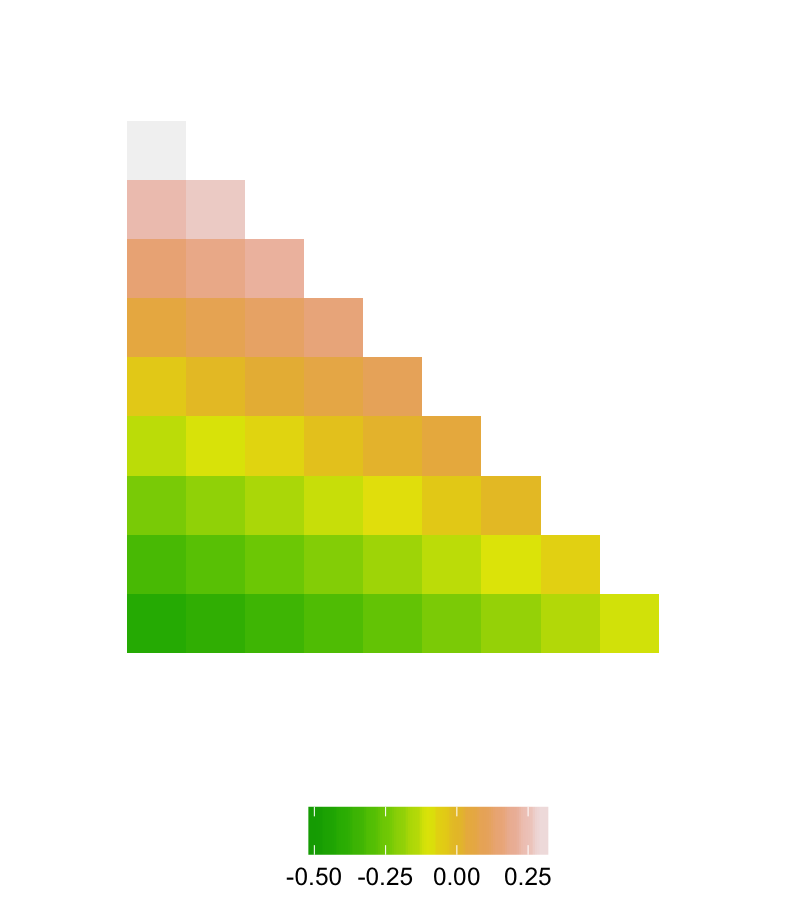
\includegraphics[width=0.25\textwidth]{img/cattle-cholesky-estimate-ggplot-phi}}%\label{fig:fitted-cholesky-decomposition-cattle-date-phi}
    \subfloat[\textit{$\log\hat{\sigma}^2\left(t\right)$}]{\label{fig:fitted-cholesky-decomposition-cattle-date-log-sigma2}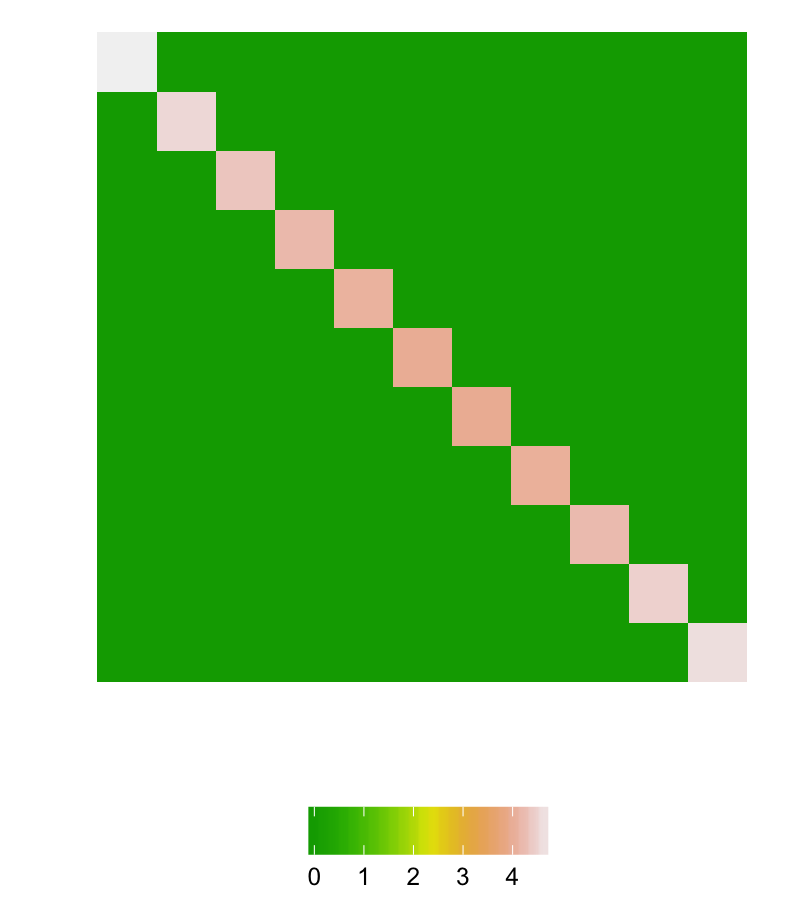
\includegraphics[width=0.25\textwidth]{img/cattle-cholesky-estimate-ggplot-log-sigma2} }
 \caption{\small{\textit{The estimated covariance matrix for the cattle weight data from treatment group A and the corresponding estimated components of the Cholesky decomposition. The generalized autoregressive coefficient function $\phi\left(t,s\right)$ and the log innovation variances $\log \sigma^2\left(t\right)$ were estimated using a tensor product cubic spline and cubic spline, respectively.}}}  \label{fig:fitted-cholesky-decomposition-cattle-date}
\end{figure}
\begin{figure}[H]
\centering
      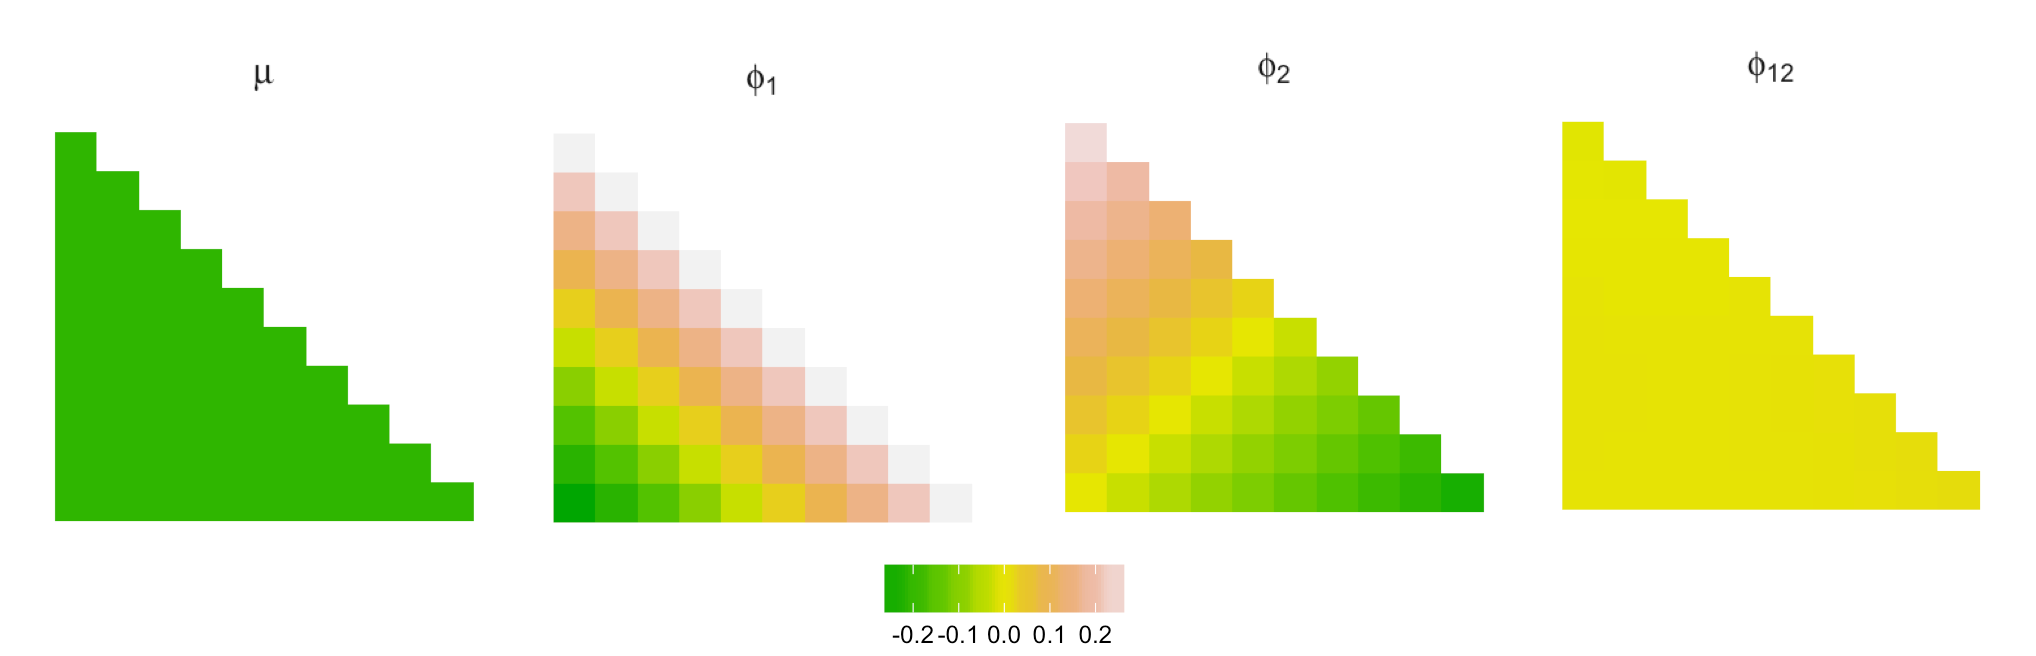
\includegraphics[width=\textwidth]{img/cattle-ssanova} 
\caption{\small{\textit{Components of the SSANOVA decomposition of the estimated generalized autoregressive coefficient function $\phi$ evaluated on the grid defined by the observed time points.}}}\label{fig:cattle-fitted-cholesky-ssanova}
\end{figure}
The size of the functional components (in terms of the squared functional norm) indicate a certain degree of concordance with the models proposed by \cite{pourahmadi1999joint}. The squared norm of the main effect of $l$ (1.914) is over twice that of the main effect of $m$ (0.790). The squared norm of the interaction term, as clearly indicated by Figure~\ref{fig:cattle-fitted-cholesky-ssanova}, is negligible in comparison to the main effects, which suggests that parameterizing $\phi$ as a univariate function of lag $l$ is a reasonable modeling choice. 
\section*{\sffamily \Large CONCLUSIONS}
We propose a general nonparametric framework for longitudinal data covariance estimation. The Cholesky decomposition supplies a reparameterization of the covariance matrix allowing for unconstrained estimation. The elements of the reparameterization can be interpreted as parameters for an autoregressive model. Our approach allows irregular, subject-specific time points by extending this regression model to a functional varying coefficient model. By reframing covariance estimation as the estimation of the functional varying coefficient function and the error variance function, our approach leverages regularization techniques that are typically reserved for function estimation.  


%\subsection*{\sffamily \large SIDEBAR}
%
%You are encouraged to include up to two sidebars (“boxed” information that is relevant to but separate from the main text), especially to highlight interdisciplinary themes. Each sidebar should be a maximum of 250 words.
%
%\section*{\sffamily \Large NOTES}
%Authors writing from a humanities or social sciences perspective may employ notes as necessary, and only if a comment or additional information is needed to expand on a citation. Notes only containing citations should be converted to references, instead. (Conversely, any references containing comments, such as “For an excellent summary of…,” should be converted to notes.) Notes should be indicated by superscript letters, both in the text and in the notes list. Citations within notes should be listed in the reference section and numbered in order.
%
%\section*{\sffamily \Large ACKNOWLEDGEMENTS}
%List contributions from individuals who do not meet the criteria for authorship (for example, to recognize contributions from people who provided technical help, collation of data, writing assistance, acquisition of funding, or a department chairperson who provided general support), with permission from the individual. Financial and material support should also be mentioned. Thanks to anonymous reviewers are not appropriate.


%Sum up the key conclusions of your review, highlighting the most promising scientific developments, directions for future research, applications, etc. The conclusion should be around 2 paragraphs, around 750 words total.


%%%%%%%%%%%%%%%%%%%%%%%%%%%%%%%%%%%%%%%%%%%%%%%%%%%%%%%%%%%%%%%%%%%%%%%%%%%%%%%%%
% BIBLIOGRAPHY
%
%% These should be cited in the text but this is a template so, of course, we don't really reference them. Please include a DOI if available.
%\nocite{coulson1960present}
%\nocite{hoffmann2008predicting}
%\nocite{koros1987separation}
%\nocite{malrieu1998quantum}
%\nocite{perdew2009some}
%\nocite{shaik2007my}

\bibliography{Master}

%\subsection*{\sffamily \Large FURTHER READING}
%%Please insert any further reading/resources here.
%For readers who may want more information on concepts in your article, provide full references and/or links to additional recommended resources (books, articles, websites, videos, datasets, etc.) that are not included in the reference section. Please do not include links to non-academic sites, such as Wikipedia, or to impermanent websites.

\end{document}

